% !TEX root = ../IntroImaging.tex

\chapter{Claude Shannon and Data Compression}
\label{chap-shannon}

\newcommand{\myfig}[3]{%
\begin{figure}[h!]\centering
#1
\caption{\label{#2}#3}
\end{figure}}

\newcommand{\imgspace}{\hspace{2mm}}
\newcommand{\tabDeux}[1]{%
\begin{tabular}{@{}c@{\imgspace}c@{}}
#1
\end{tabular}}
%
\newcommand{\tabTrois}[1]{%
\begin{tabular}{@{}c@{\imgspace}c@{\imgspace}c@{}}
#1
\end{tabular}}
%
\newcommand{\tabQuatre}[1]{%
\begin{tabular}{@{}c@{\imgspace}c@{\imgspace}c@{\imgspace}c@{}}
#1
\end{tabular}}


\newcommand{\BL}[1]{{\color{blue}{#1}}}
\newcommand{\RE}[1]{{\color{red}{#1}}}
\newcommand{\GR}[1]{{\color{magenta}{#1}}}
\newcommand{\WH}[1]{{\color{white}{#1}}}
\newcommand{\LG}[1]{{\color{lightgray}{#1}}}



\newcommand{\mot}{\BL{v}}
\newcommand{\Mot}{\BL{V}}
\newcommand{\differ}{\GR{d}}
\newcommand{\Differ}{\GR{D}}
%
\newcommand{\LongMoy}{\Ll}
\newcommand{\LongTot}{\bar\Ll}


\newcommand{\mylink}[1]{\footnote{\url{#1}}}



%\newcommand{\myparagraph}[1]{\paragraph{#1.}}
%\renewcommand{\myparagraph}[1]{\subsection{#1}}
 
	The vast majority of data (text, sound, image, video, etc.) is stored and manipulated in digital form, that is, using integers which are converted into a succession of bits $\RE{0}$ and $\RE{1}$). Conversion from the continuous analog world to these discrete numerical representations is described by the theory developed by Claude Shannon (April 30, 1916 - February 24, 2001), the founding father of the theory of information. The impact of this theory on our society is absolutely colossal. Yet his name is almost unknown to the general public. The centenary of the birth of Claude Shannon is therefore a good excuse to present the work of a very great scientist.


%%%%%%%%%%%%%%%%%%%%%%%%%%%%%%%%%%%%%%%%%%%%%%%%%%%%%%%%%%%%%%%%%%%%%%%%%%%%%%%%%%
%%%%%%%%%%%%%%%%%%%%%%%%%%%%%%%%%%%%%%%%%%%%%%%%%%%%%%%%%%%%%%%%%%%%%%%%%%%%%%%%%%
%%%%%%%%%%%%%%%%%%%%%%%%%%%%%%%%%%%%%%%%%%%%%%%%%%%%%%%%%%%%%%%%%%%%%%%%%%%%%%%%%%
\section{Numeric Data and Coding}

In the digital world that surrounds us, all data (images, films, sounds, texts, etc.) are coded in the form of a succession of $\RE{0}$ and $\RE{1}$. This encoding is not limited to storage on computers, it is also central for communications over the internet (email, \guill{streaming} video \mylink{https://en.wikipedia.org/wiki/Streaming} , etc.) as well as for applications as diverse as music players, e-readers or mobile phones.

However, data (eg text, sounds, images, or videos) is initially represented as a succession of \textit{symbols}, which are not necessarily $\RE{0}$ or of $\RE{1}$. For example, for the case of a text, the symbols are the letters of the alphabet. For the case of images, these are the values of the pixels. It is therefore necessary to be able to convert this sequence of symbols into a sequence of $\RE{0}$ and $\RE{1}$. It is also necessary to be able to do it in an economical way, that is to say using the shortest possible sequence. This is crucial in order to be able to store this data efficiently on a hard disk, or to transmit them quickly on the Internet. This problem of \textit{compression} has become a major issue because the stored and transmitted data grow exponentially.

The theory developed by Claude Shannon describes the theoretical and algorithmic bases of this coding. He mathematically formalized the three key stages of conversion from the analog world to the digital world:
\begin{itemize}
\item[(i)] \textit{sampling} \mylink{https://en.wikipedia.org/wiki/sampling (signal)}, which allows you to switch from continuous data to a succession of numbers;
%
\item[(ii)] \textit{coding} \mylink{https://en.wikipedia.org/wiki/Compression_Data} (also known as compression), which allows you to move to a more compact sequence of $\RE{0}$ and $\RE{1}$(called binary code);
%
\item[(iii)] \textit{error-correcting code} \mylink{https://en.wikipedia.org/wiki/Code_Corrector}, which makes code robust to errors and attacks.
\end{itemize}

For each of these steps, Claude Shannon has established \guill{upper bounds} in~\cite{Shannon1948,shannon1949}, under precise assumptions about the data and the transmission channel. These performance bounds set limits that can not be exceeded, regardless of the method used. For example, for encoding phase (ii), this bound corresponds to the minimum theoretical size of the binary messages making it possible to code the desired information. In the second half of the 20th century, efficient calculation methods and algorithms were developed to reach the limits of Shannon, leading to the 21st century on the explosion of the digital age. This article focuses on part (ii) and presents the basics of data compression as defined by Claude Shannon. For part (iii), one can for example consult this article of images of the mathematics \mylink{http://images.math.cnrs.fr/Qui-est-ce}.

You can find at the end of this article a glossary summarizing the most important terms.


%%%%%%%%%%%%%%%%%%%%%%%%%%%%%%%%%%%%%%%%%%%%%%%%%%%%%%%%%%%%%%%%%%%%%%%%%%%%%%%%%%
%%%%%%%%%%%%%%%%%%%%%%%%%%%%%%%%%%%%%%%%%%%%%%%%%%%%%%%%%%%%%%%%%%%%%%%%%%%%%%%%%%
%%%%%%%%%%%%%%%%%%%%%%%%%%%%%%%%%%%%%%%%%%%%%%%%%%%%%%%%%%%%%%%%%%%%%%%%%%%%%%%%%%
\section{Encoding and decoding}

We will now describe and study the transformation (coding) from the sequence of $\{\BL{0,1,2,3}\}$ symbols to a binary code, that is, a sequence of $\RE{0}$ and $\RE{1}$.


%%%%%%%%%%%%%%%%%%%%%%%%%%%%%%%%%%%%%%%%%%%%%%%%%% %%%%%%%%%%%%%%%%%%%%%%%%%%%%%%%%
\subsection{Example of an image}

In the rest of this article, I will illustrate my remarks using grayscale images. Such an image is composed of pixels. To simplify, we will consider only pixels with 4 levels of gray:
\begin{itemize}
\item $\BL{0}$: black, 
\item $\BL{1}$: dark gray,
\item $\BL{2}$: light gray,
\item $\BL{3}$: white.
\end{itemize}

However, all that will be described hereafter is generalized to an arbitrary number of gray levels (in general, the images that are found on the internet have 256 levels) and even to the color images (which can be decomposed in 3 monochrome images, the red, green and blue components).

Figure~\ref{fig-image-zoom} shows an example of an image with 4 levels of gray, with a zoom on a subset of $5 \times 5$ pixels.

\myfig{
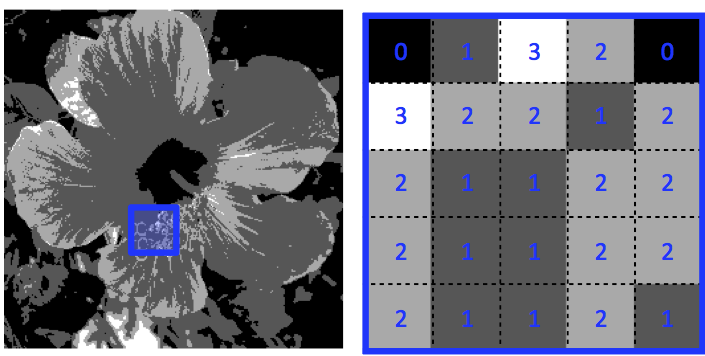
\includegraphics[width=.6\linewidth]{codage/codage-pxl}
}{fig-image-zoom}{A greyscale image and a zoom on a square of $5 \times 5$ pixels}


We will focus on this set of 25 pixels (the rest of the image is treated in the same way). If we put the corresponding values one after the other, we get the following sequence of symbols, which are numbers between $\BL{0}$ and $\BL{3}$
$$
	(\BL{0, 1, 3, 2, 0, 3, 2, 2, 1, 2, 2, 1, 1, 2, 2, 2, 1, 1, 2, 2, 2, 1, 1, 2, 1}).
$$

%%%%%%%%%%%%%%%%%%%%%%%%%%%%%%%%%%%%%%%%%%%%%%%%%% %%%%%%%%%%%%%%%%%%%%%%%%%%%%%%%%
\subsection{Uniform Coding}

The coding step therefore proceeds by associating to each of the symbols $\{\BL{0,1,2,3}\}$ a code word, which is a sequence of $\RE{0}$ and $\RE{1}$.

One possible strategy is to use coding
$$
\BL{0} \mapsto \RE{00}, \quad
\BL{1} \mapsto \RE{01}, \quad
\BL{2} \mapsto \RE{10}, \quad
\BL{3} \mapsto \RE{11}.
$$
This is a particular case of \textit{uniform} coding, which associates with each symbol a code word of fixed length (here of constant length 2).

Thus the sequence of $(\BL{0, 1, 3})$ symbols is coded as
$$
	(\BL{0, 1, 3}) \overset{\text{codage}}{\longmapsto}
	(\RE{00,01,11}) \overset{\text{regroupement}}{\longmapsto}
	\RE{000111}.
$$
The complete sequence of symbols corresponding to the image of $ 5 \times 5 $pixels shown above
will give the code
$$
  \RE{00011110001110100110100101101010010110101001011001}.
$$
The length (ie the number of $\BL{0}$ and $\BL{1}$) in the sequence $\BL{0}$ and $\BL{1}$ used to encode a message is measured in number of \textit{bits}. Using the previous uniform coding, which uses 2 bits per symbols, as one must code 25 symbols, a length
$$
	\mathcal{\bar L} = 25 \times 2 = 50 \text{ bits}
$$
The \textit{bit} (\guill{binary digit}) is the fundamental unit of information, and was introduced by John Tukey \mylink{https://en.wikipedia.org/wiki/John_Tukey} was a collaborator of Claude Shannon.



%%%%%%%%%%%%%%%%%%%%%%%%%%%%%%%%%%%%%%%%%%%%%%%%%% %%%%%%%%%%%%%%%%%%%%%%%%%%%%%%%%
\subsection{Logarithm and Uniform Coding}

If the number $ N $ of possible symbols (in this case $N=4$) is a power of $2$, that is $N=2^\ell$(here $N=4=2^2$ so that $\ell=2$), one can always construct such a \textit{uniform} code where one associates to each symbol its binary writing. We have given the example of the uniform coding of $N=4$ symbols, and the case of $N=8$  (thus $\ell=$ 3) symbols corresponds to the coding
$$
\BL{0} \mapsto \RE{000}, \quad
\BL{1} \mapsto \RE{001}, \quad
\BL{2} \mapsto \RE{010}, \quad
\BL{3} \mapsto \RE{011},
$$
$$
\BL{4} \mapsto \RE{100}, \quad
\BL{5} \mapsto \RE{101}, \quad
\BL{6} \mapsto \RE{110}, \quad
\BL{7} \mapsto \RE{111}.
$$

This binary script has a length $\ell $, which is called the logarithm in base of 2 \mylink{https://en.wikipedia.org/wiki/Binary_Logarithm} of $ N $, which is noted
$$
N=2^\ell \quad \Longleftrightarrow \quad \log_2(N) \eqdef \ell.
$$
The definition of $\log_2(x)$ also extends to the case where $x$ is not a power of 2, using the definition $\log_2(x) \eqdef \ln(x)/\ln(2)$, where $\ln$ is the \textit{natural logarithm}.
%
In this case, $\log_2(x)$ is not an integer. For a strictly positive real number $x$, the logarithm satisfies
$\log_2(1/x)=-\log_2(x)$, so for example, we have $\log_2(1/4)=-\log_2(4)=2$.



%%%%%%%%%%%%%%%%%%%%%%%%%%%%%%%%%%%%%%%%%%%%%%%%%%%%%%%%%%%%%%%%%%%%%%%%%%%%%%%%%%
\subsection{Variable-length encoding}

An important question is whether we can do better (that is, use fewer bits to code the same sequence of symbols). For example, the following coding may be used instead of a uniform code
$$
\BL{0} \mapsto \RE{001}, \quad
\BL{1} \mapsto \RE{01}, \quad
\BL{2} \mapsto \RE{1}, \quad
\BL{3} \mapsto \RE{000}.
$$
With such coding, the $(\BL{0, 1, 3})$ symbol sequence is coded as
$$
	(\BL{0, 1, 3}) \overset{\text{codage}}{\longmapsto}
	(\RE{001,01,000}) \overset{\text{regroupement}}{\longmapsto}
	\RE{00101000}.
$$
The complete sequence of symbols corresponding to the image of $ 5 \times $ 5 pixels
will give the code
$$
  \RE{001010001001000110111010111101011110101101}.
$$
The length of the binary code obtained is therefore now
$$
\mathcal{\bar L} = 42 \text{bits}
$$
This shows that it is therefore possible to do better than with a \textit{uniform} coding using a \textit{variable} coding, which associates a variable length code with each symbol.

It is also possible to define the average number of bits per symbol $\mathcal{L}$, which is computed, here for a sequence of 25 symbols, as
$$
	\mathcal{L} \eqdef \frac{ \mathcal{\bar L} }{25} = \frac{42}{25} = 1.68 \text{ bits.}
$$
Compared to a uniform coding, it is seen that the average number of bits per symbol has changed from $\log_2(N)=2 \text{ bits}$ to $ 1.68 \text{ bits}$.




%%%%%%%%%%%%%%%%%%%%%%%%%%%%%%%%%%%%%%%%%%%%%%%%%% %%%%%%%%%%%%%%%%%%%%%%%%%%%%%%%%
\subsection{Encoding prefix and decoding}

These codings, uniform or of variable length, would be of no interest if we did not ensure that the message obtained is \textit{decodable}, ie we can find the sequence of symbols at the origin of a binary code. All encodings do not allow for this reverse path.

For uniform encodings, such as coding
$$
\BL{0} \mapsto \RE{00}, \quad
\BL{1} \mapsto \RE{01}, \quad
\BL{2} \mapsto \RE{10}, \quad
\BL{3} \mapsto \RE{11}.
$$
it is sufficient to separate the sequence of bits into packets of length $\log_2(N)$(here $ N=$ 4 and $\log_2(N)=$ 2) and use the encoding table in the opposite direction.
Thus, the $\RE{000111}$ binary code is decoded as
$$
	\RE{000111} \overset{\text{s�paration}}{\longmapsto}
	(\RE{00,01,11})  \overset{\text{d�codage}}{\longmapsto}
	(\BL{0, 1, 3}).
$$

On the other hand, if we consider the coding
$$
\BL{0} \mapsto \RE{0}, \quad
\BL{1} \mapsto \RE{10}, \quad
\BL{2} \mapsto \RE{110}, \quad
\BL{3} \mapsto \RE{101},
$$
then the bit sequence $\RE{1010}$can be decoded in two ways:
$$
	\RE{1010}
	\overset{\text{s�paration}}{\longmapsto}
	(\RE{10, 10})
	\overset{\text{d�codage}}{\longmapsto}
	(\BL{1, 1}),
$$
or
$$
	\RE{1010}
	\overset{\text{s�paration}}{\longmapsto}
	(\RE{101, 0})
	\overset{\text{d�codage}}{\longmapsto}
	(\BL{3, 0}).
$$
This means that this sequence can be decoded either as the sequence $(\BL{1, 1})$, or as the $(\BL{3, 0})$ sequence.
Note that the $\RE{10}$ encoding word used to encode $\BL{1}$ is the beginning of the $\RE{101}$ word used to encode $\BL{3}$.

To be able to do the decoding in an unambiguous way, it is enough that no word of the coding is the beginning of another word. When this condition is satisfied, we speak of \textit{prefix} \mylink{https://en.wikipedia.org/wiki/Prefix_Code}
and it is therefore possible to carry out the decoding step by step.
It is easily verified that this is indeed the case for the non-uniform coding already considered previously
$$
\BL{0} \mapsto \RE{001}, \quad
\BL{1} \mapsto \RE{01}, \quad
\BL{2} \mapsto \RE{1}, \quad
\BL{3} \mapsto \RE{000}.
$$
The progressive decoding of the symbol message of the pixels of the image is carried out as follows:
$$
	\RE{001}\LG{010001001000110111010111101011110101101}
		\longrightarrow  \text{ d�code } \BL{0}
$$
$$
	\WH{0}\BL{0}\WH{1}\RE{01}\LG{0001001000110111010111101011110101101}
			\longrightarrow  \text{ d�code } \BL{1}
$$
$$
	\WH{0}\BL{0}\WH{1}\BL{1}\WH{0}\RE{000}\LG{1001000110111010111101011110101101}
	\longrightarrow  \text{ d�code } \BL{3}
$$
$$
	\WH{0}\BL{0}\WH{1}\BL{1}\WH{0}\WH{0}\BL{3}\WH{0}\RE{1}\LG{001000110111010111101011110101101}
		\longrightarrow  \text{ d�code } \BL{2} \ldots
$$

%%%%%%%%%%%%%%%%%%%%%%%%%%%%%%%%%%%%%%%%%%%%%%%%%% %%%%%%%%%%%%%%%%%%%%%%%%%%%%%%%%
\subsection{Codes and Trees}
\label{sec-arbres}

As shown in the figure~\ref{fig-trees}, in the top left, it is possible to place the set of binary codes of less than $\ell $ bits in a tree of depth $\ell + 1 $. The $ 2^\ell $ words of length exactly $\ell $ occupy the sheets, and the shorter words are the inner nodes.

\myfig{
\tabTrois{
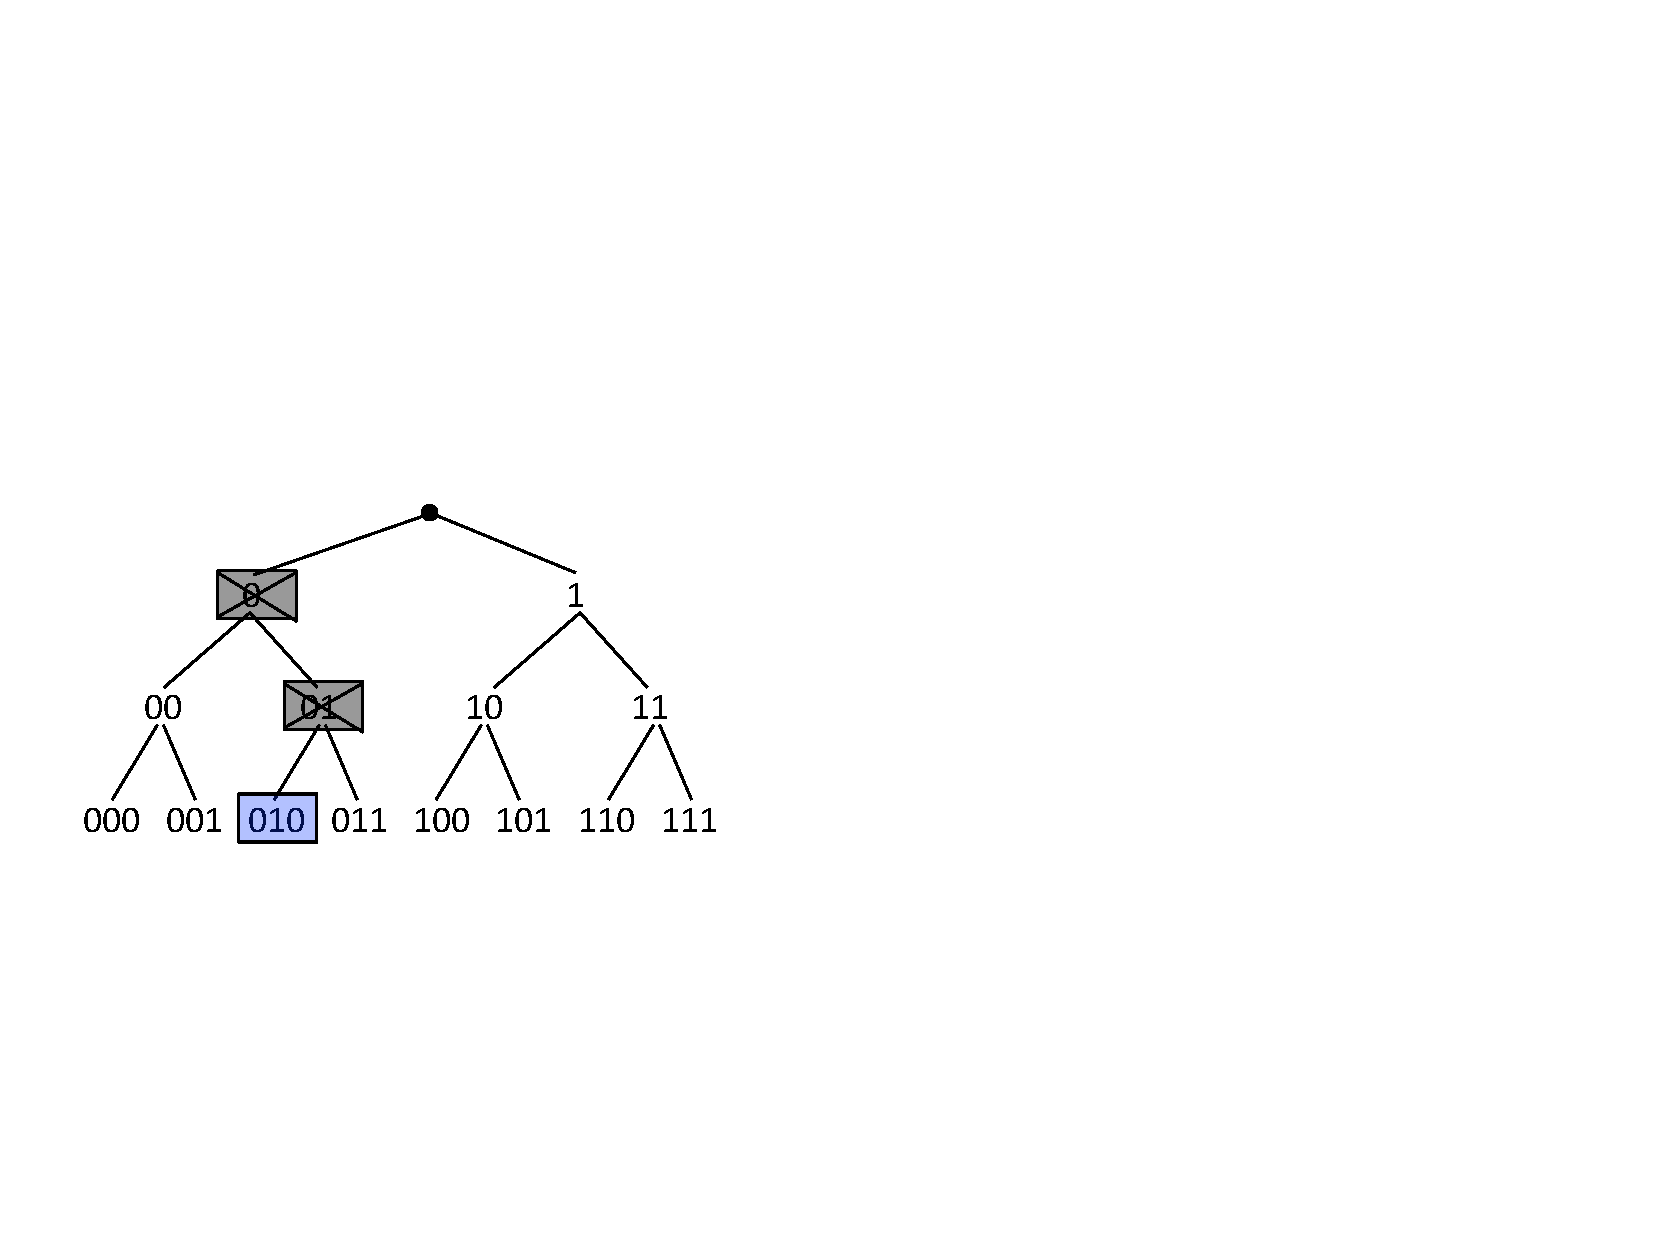
\includegraphics[width=.45\linewidth]{arbres/codage-prefixe}&
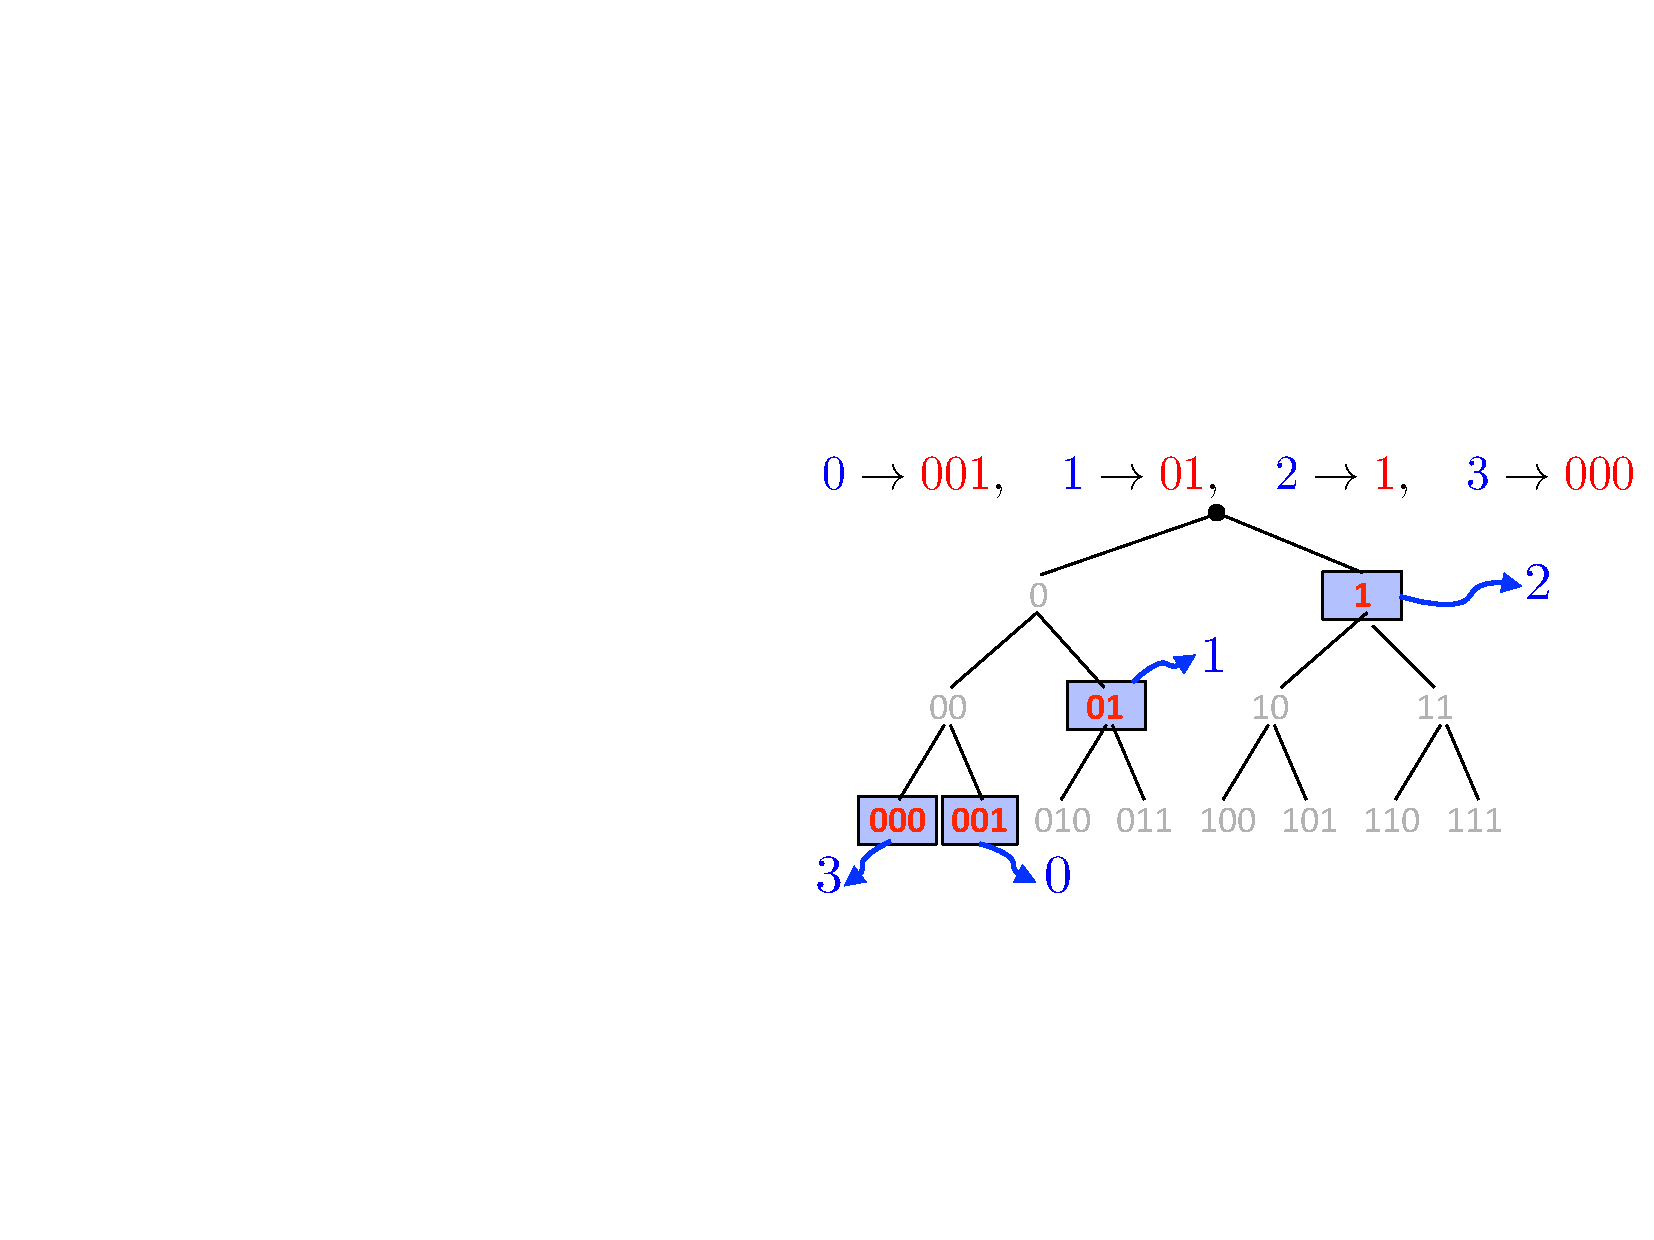
\includegraphics[width=.45\linewidth]{arbres/arbre-exemple}
}
}{fig-trees}{Left: complete tree of all codes of length 3; right: sample encoding prefix.}

The prefix encodings are then represented as the leaves of the subtrees of this complete tree. The figure~\ref{fig-trees}, top right, shows which subtree corresponds to the variable-length code
$$
\BL{0} \mapsto \RE{001}, \quad
\BL{1} \mapsto \RE{01}, \quad
\BL{2} \mapsto \RE{1}, \quad
\BL{3} \mapsto \RE{000}.
$$

Once a prefix encoding has been represented as a binary subtree, the decoding algorithm is particularly simple to implement. When decoding is begun, one moves to the root, and descends to each new bit read either to the left (for a $\RE{0}$) or to the right (for a $\RE{1}$ ). When one reaches a sheet of the subtree, one then sends the word of the code corresponding to this sheet, and one restarts to the root. The previous figure shows the decoding process.


%%%%%%%%%%%%%%%%%%%%%%%%%%%%%%%%%%%%%%%%%%%%%%%%%% %%%%%%%%%%%%%%%%%%%%%%%%%%%%%%%%
%%%%%%%%%%%%%%%%%%%%%%%%%%%%%%%%%%%%%%%%%%%%%%%%%% %%%%%%%%%%%%%%%%%%%%%%%%%%%%%%%%
%%%%%%%%%%%%%%%%%%%%%%%%%%%%%%%%%%%%%%%%%%%%%%%%%% %%%%%%%%%%%%%%%%%%%%%%%%%%%%%%%%
\section{The Shannon Bound}

After describing the coding techniques, we will now explain the Shannon theory, which analyzes the performance of these techniques (ie the number of bits needed for coding) by performing a random modeling of the message to be coded which is composed of a particular sequence of symbols).


%%%%%%%%%%%%%%%%%%%%%%%%%%%%%%%%%%%%%%%%%%%%%%%%%% %%%%%%%%%%%%%%%%%%%%%%%%%%%%%%%%
\subsection{Minimum length code and random modeling}

The use of variable length prefix encoding shows that an average number of bits $\mathcal{L}$can be obtained than the number $\log_2(N)$ of bits obtained by a uniform code. The fundamental question, both on a theoretical and practical level, is whether we can find a prefix coding giving rise to a minimum number of bits per symbol.

This question is badly asked, because its answer depends on the message to be coded, and this message is generally unknown a priori. A model is therefore needed to describe possible messages. The fundamental idea introduced by Claude Shannon is to use a probabilistic model: we do not know what messages we will have to code, but we assume that we know the probability of appearance of the symbols composing this message.

Shannon assumes that the symbols that make up the modeled message are drawn \textit{independently} \mylink{https://en.wikipedia.org/wiki/Independencies_ (probability)}
according to a random variable $\Mot$(the source of the message). This means that the symbols composing the modeled message are independent random variables with the same distribution as $\Mot$.

%%%%%%%%%%%%%%%%%%%%%%%%%%%%%%%%%%%%%%%%%%%%%%%%%% %%%%%%%%%%%%%%%%%%%%%%%%%%%%%%%%
\subsection{Empirical Frequencies}

In order to apply this probabilistic model to a given message, we will act as if we randomly draw each symbol one after the other according to probabilities identical to the frequencies observed (on average) in the case studied.

This means that we impose that the distribution of the $\Mot$ source to be equal to the empirical frequencies observed in the message.
%
Empirical frequencies $(p_{\BL{0}},p_{\BL{1}},p_{\BL{2}},p_{\BL{3}})$ are the frequency of appearance of the different symbols $(\BL{0,1,2,3})$. 
%
For the set of the 25 pixels of the grayscale image
$$
	(\BL{0, 1, 3, 2, 0, 3, 2, 2, 1, 2, 2, 1, 1, 2, 2, 2, 1, 1, 2, 2, 2, 1, 1, 2, 1}), 
$$
the frequency $p_{\BL{1}}$ is equal to $ 9/25 $ because the symbol $\BL{1}$ appears $ 9 $ times and it is desired to encode a sequence of 25 symbols. The list of empirical frequencies for this sequence of symbols is thus
$$
  	p_{\BL{0}} = \tfrac{2}{25}, \quad
	p_{\BL{1}} = \tfrac{9}{25}, \quad
	p_{\BL{2}} = \tfrac{12}{25}, \quad
	p_{\BL{3}} = \tfrac{2}{25}.
$$

The random modeling therefore imposes on the variable $\Mot$ to have for probability distribution $(p_{\BL{0}},p_{\BL{1}},p_{\BL{2}},p_{\BL{3}})$, ie the probability that a symbol of the modeled message (assumed to be generated by the $\Mot$ source) is $\mathbb{P}(\Mot=\mot) = p_{\mot}$.

This is an important example of modeling, which is of course not always relevant but allows a fine analysis of the problem. For example, in the case of an image, if a pixel is black, the next one is likely to be black, even if the overall black frequency is low. This defeats the independence hypothesis (the \guill{Information Transformation} section details this example).



%%%%%%%%%%%%%%%%%%%%%%%%%%%%%%%%%%%%%%%%%%%%%%%%%% %%%%%%%%%%%%%%%%%%%%%%%%%%%%%%%%
\subsection{Entropy} 

In order to answer the coding problem with a minimum average number of bits, Shannon introduced a fundamental mathematical object: \textit{entropy}\mylink{https://en.wikipedia.org/wiki/Entropy}.
Entropy was invented by Ludwig Boltzmann \mylink{https://en.wikipedia.org/wiki/Ludwig_Boltzmann}
in the context of thermodynamics \mylink{https://en.wikipedia.org/wiki/Entropie_ (thermodynamics)}
and this concept was taken up by Claude Shannon to develop his theory of information.
The entropy of the distribution of the source $\Mot$ is defined by the formula
$$
	\mathcal{H}_\Mot \eqdef -\sum_{\mot=0}^{N-1} p_{\mot} \times \log_2(p_{\mot}).
$$
This formula means that we sum up for all possible $\mot$ symbols the frequency of occurrence $p_{\mot}$ of the symbol $\mot$ multiplied by the logarithm $\log_2(p_{ \mot})$ of this frequency, then take the opposite (minus sign) of the number obtained.

As the logarithm is an increasing function, and as $\log_2(1)=0$, we have $\log_2(p_{\mot}) \leq 0$ because $p_{\mot}$ is always less than $1$). The minus sign before the formula defining the entropy ensures that this quantity is always positive.

In our case, we have $N=4$ values for the symbols, and we use the formula
$$
	\mathcal{H}_\Mot \eqdef
- p_{\BL{0}} \times \log_2(p_{\BL{0}})
- p_{\BL{1}} \times \log_2(p_{\BL{1}})
- p_{\BL{2}} \times \log_2(p_{\BL{2}})
- p_{\BL{3}} \times \log_2(p_{\BL{3}}).
$$
Note that if $p_{\mot}=0$, then the convention $p_{\mot} \times \log_2(p_{\mot})=0 \times \log_2(0)=$ 0. This convention means that null probabilities (ie, impossible events) are not taken into account in this formula. Moreover, it is consistent with the limit value of the function $x \mapsto x \ln(x)$ at $x=0$.



The goal of entropy is to quantify the uncertainty on possible symbol sequences generated by the $\Mot$ source. We can show that the entropy verifies
$$
	0 \leq \mathcal{H}_\Mot \leq \log_2(N).
$$
The two extreme values thus correspond to respective minimum and maximum uncertainties.

\myfig{
\tabQuatre{
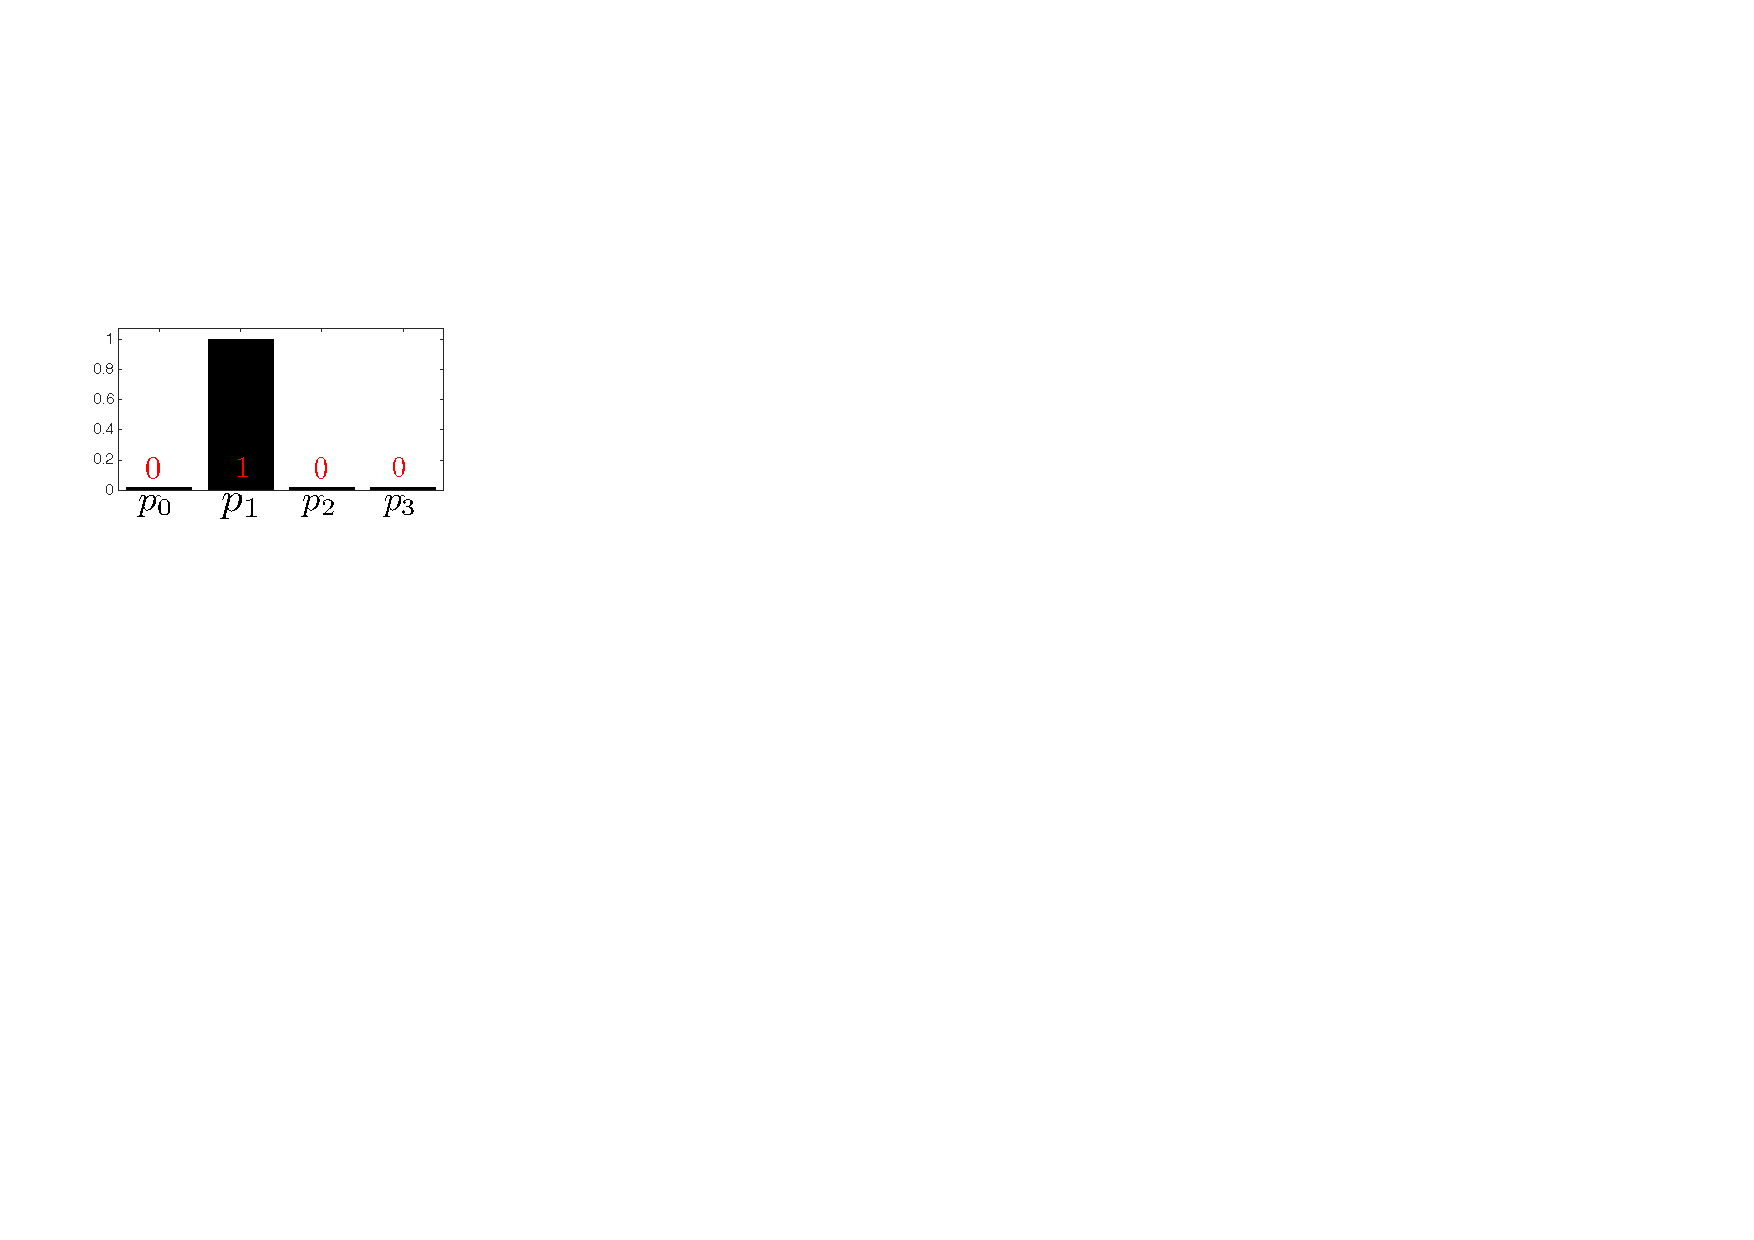
\includegraphics[width=.3\linewidth]{entropie/histo-1}&
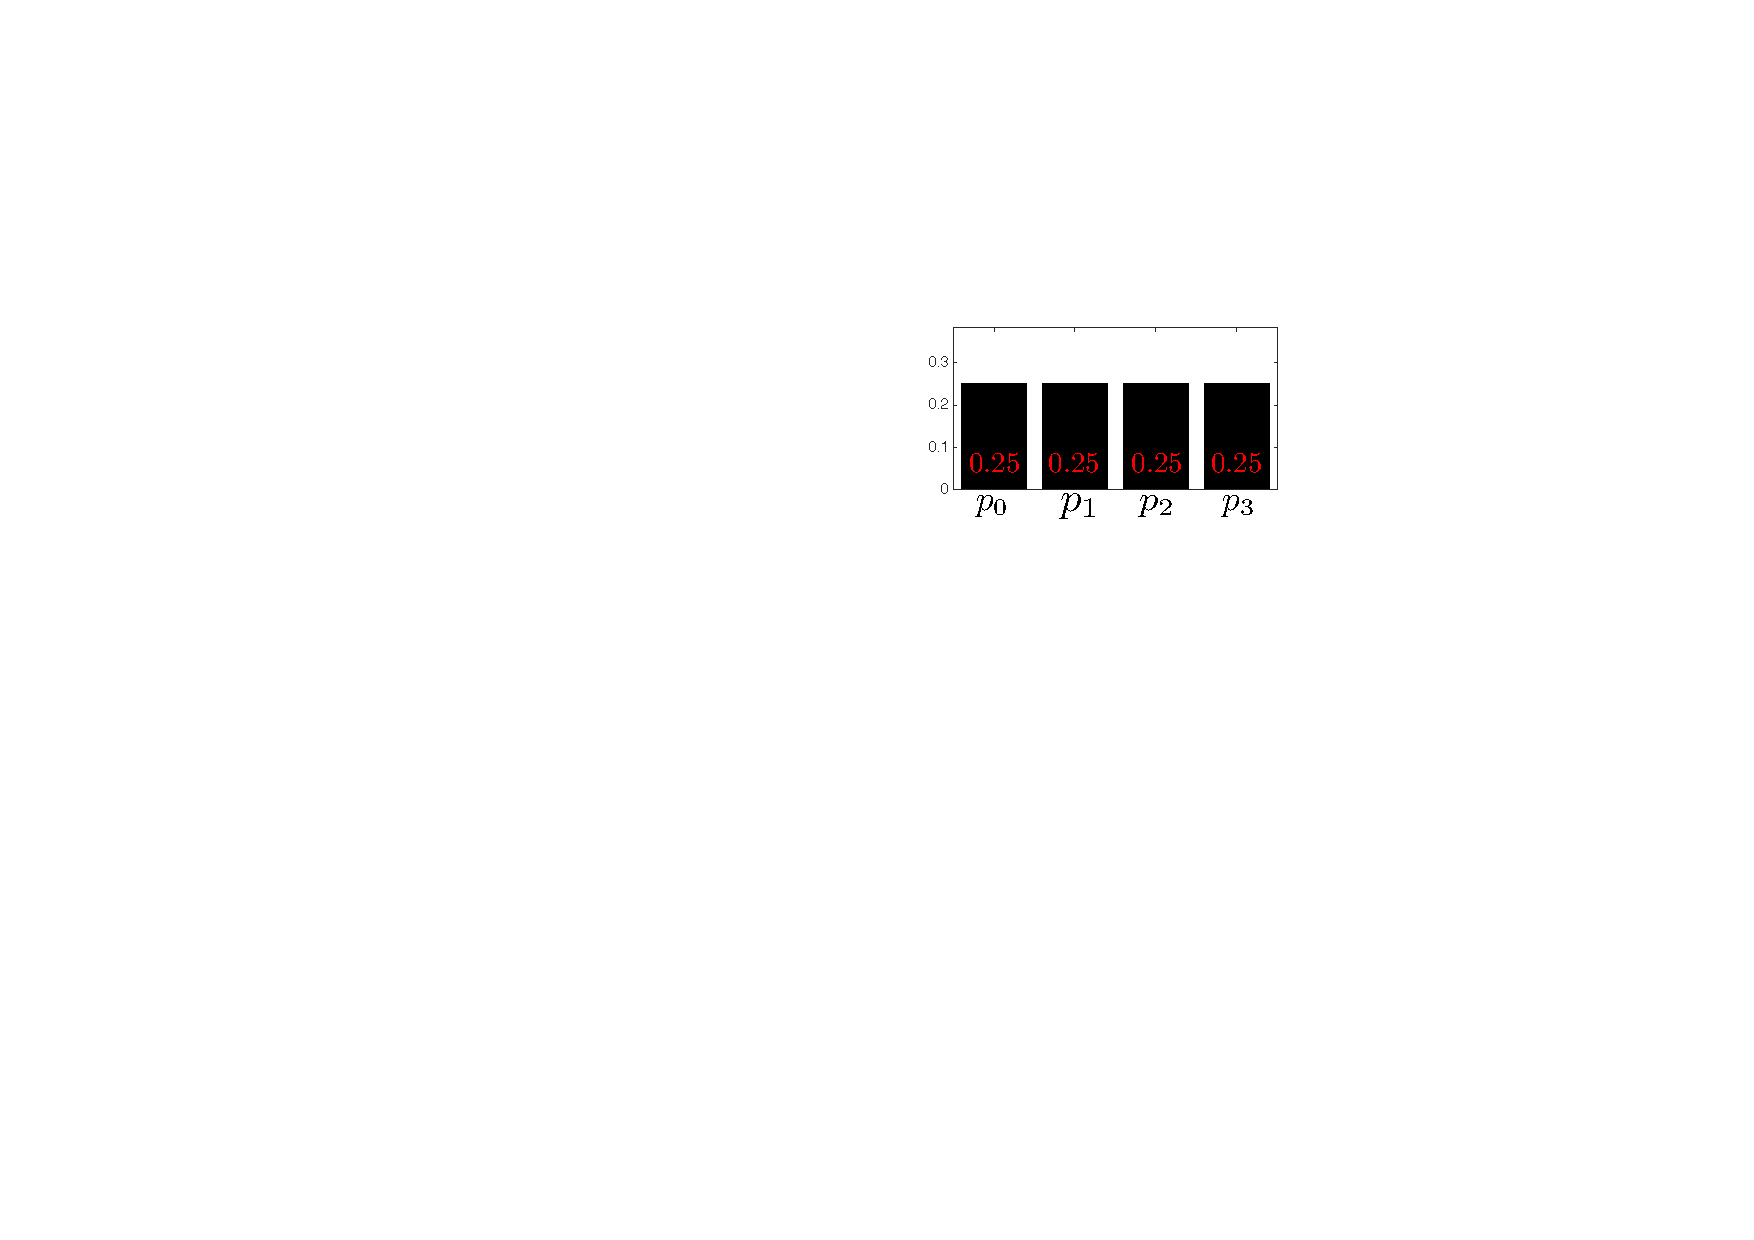
\includegraphics[width=.3\linewidth]{entropie/histo-3}&
\includegraphics[width=.3\linewidth]{entropie/histo-sub}\\
$\Hh_{\Mot}=0$ & $\Hh_{\Mot}=\log_2(2)=1$ &  $\Hh_{\Mot} = 1.62$
}
}{fig-histo-entropy}{Three examples of probability distributions with corresponding entropies.}


\begin{itemize}
%%%%%%%%%%%%%%%%%%%%%%%%%%%%%%%%%%%%%%%%%%%%%%%%%%%%%%%%%%%%%%%%%%%%
\item \textbf{Minimal entropy}
%
 The entropy $\mathcal{H}_\Mot=0$  is minimal when the frequencies $p_{\mot}$ are all null except one. The left-handed figure~\ref{fig-histo-entropy} shows the case where $p_{\BL{1}}=1$ and all other probabilities are null.


In this case,
$$
	\mathcal{H}_\Mot = - 0 \times \log_2(0) - 1 \times \log_2(1) - 0 \times \log_2(0)- 0 \times \log_2(0) = 0, 
$$
where we recall that $\log_2(1)=0$ and that by convention we have $ 0 \times \log_2(0)=0$.
This corresponds to the modeling of a constant sequence of symbols, and the source will generate, for example, with probability 1 the following sequence of 25 symbols
$$
		(\BL{0, 0, 0, 0, 0, 0, 0, 0, 0, 0, 0, 0, 0, 0, 0, 0, 0, 0, 0, 0, 0, 0, 0, 0, 0}).
$$
%%%%%%%%%%%%%%%%%%%%%%%%%%%%%%%%%%%%%%%%%%%%%%%%%%%%%%%%%%%%%%%%%%
\item \textbf{Maximum entropy}
%
On the other hand, $\mathcal{H}_\Mot=\log_2(N)$ is maximal when all frequencies are equal, $p_{\mot}=1/N $.
In our case where $N=4$, we have
$$
 \mathcal{H}_\Mot =
 		-\tfrac{1}{4} \times \log_2(\tfrac{1}{4})
  	-\tfrac{1}{4} \times \log_2(\tfrac{1}{4})
		-\tfrac{1}{4} \times \log_2(\tfrac{1}{4})
		-\tfrac{1}{4} \times \log_2(\tfrac{1}{4})
		= \log_2(4) = 2,
$$
where $\log_2(1/x)=-\log_2(x)$ is used and therefore in particular $\log_2(\frac{1}{4})=-\log_2(4)$. The following figure~\ref{fig-histo-entropy}, center, shows the histogram corresponding to this case.

This situation corresponds intuitively to the modeling of a sequence maximally \textit{uncertain}.
Here, for example, are two sequences of symbols generated by such a source $\Mot$
$$
  (\BL{2, 2, 1, 1, 3, 0, 3, 3, 3, 0, 1, 1, 2, 0, 2, 0, 2, 1, 3, 2, 0, 2, 2, 1, 3}),
$$
$$
  (\BL{3, 3, 1, 2, 0, 0, 2, 2, 1, 3, 2, 2, 3, 3, 2, 0, 0, 3, 0, 1,  3, 0, 1, 1, 2}).
$$

%%%%%%%%%%%%%%%%%%%%%%%%%%%%%%%%%%%%%%%%%%%%%%%%%%%%%%%%%%%%%%%%%%
\item \textbf{Intermediate entropy}
%
The intermediate situations between these two extremes correspond to intermediate entropies.
For example, we can consider the distribution of the 25 pixels considered at the beginning of this article, which correspond to the message
$$
	(\BL{0, 1, 3, 2, 0, 3, 2, 2, 1, 2, 2, 1, 1, 2, 2, 2, 1, 1, 2, 2, 2, 1, 1, 2, 1}).
$$
For this distribution, we recall that we have the probabilities
$$
  p_{\BL{0}} = \tfrac{2}{25}, \quad
	p_{\BL{1}} = \tfrac{9}{25}, \quad
	p_{\BL{2}} = \tfrac{12}{25}, \quad
	p_{\BL{3}} = \tfrac{2}{25},
$$
the figure~\ref{fig-histo-entropy}, right, shows the histogram corresponding to these values.


The entropy then
$$
	\mathcal{H}_\Mot =
	  -\tfrac{2}{25} \times \log_2(\tfrac{2}{25})
		-\tfrac{9}{25} \times \log_2(\tfrac{9}{25})
		-\tfrac{12}{25}\times \log_2(\tfrac{12}{25})
		-\tfrac{2}{25}\times \log_2(\tfrac{2}{25}) \approx 1.62,
$$
which corresponds to a \guill{intermediate} value of the entropy.
\end{itemize}


%%%%%%%%%%%%%%%%%%%%%%%%%%%%%%%%%%%%%%%%%%%%%%%%%% %%%%%%%%%%%%%%%%%%%%%%%%%%%%%%%%
\subsection{Average number of bits of a source}

In the following, we denote $c_{\mot}$ the code associated with a symbol $\mot$. The length (i.e. the number of bits) of each word $c_{\mot}$ of code is denoted $L(c_{\mot})$. For uniform coding, then the length is constant $L(c_{\mot})=\log_2(N)$.
On the other hand, if we take the example of variable coding
$$
	\BL{0} \mapsto c_{\BL{0}} \eqdef \RE{001}, \quad
	\BL{1} \mapsto c_{\BL{1}} \eqdef \RE{01}, \quad
	\BL{2} \mapsto c_{\BL{2}} \eqdef \RE{1}, \quad
	\BL{3} \mapsto c_{\BL{3}} \eqdef \RE{000},
$$
then $L(c_{\BL{0}})=L(\RE{001})=$ 3.

It can be seen that the average bit number $\mathcal{L}$ of the encoding of a message can be calculated using the empirical frequencies as follows:
$$
	\mathcal{L} = \sum_{\mot=0}^{N-1} p_{\mot} \times L(c_{\mot}).
$$
This formula means that we sum up for all possible $\mot$ symbols the frequency of occurrence $p_{\mot}$ of the symbol multiplied by the length $L(c_{\mot})$ of the code word $c_{\mot}$. For example, in our case, for $ N=$ 4, we have the formula
$$
	\mathcal{L} =
		p_{\BL{0}} \times L(c_{\BL{0}}) +
		p_{\BL{1}} \times L(c_{\BL{1}}) +
		p_{\BL{2}} \times L(c_{\BL{2}}) +
		p_{\BL{3}} \times L(c_{\BL{3}}).
$$

As part of the random modeling using a $\Mot$ source, we will write $\mathcal{L}_\mot$ this average bit number, which is associated with the source $\Mot$ having the distribution $(p_ \mot)_{\mot}$.


%%%%%%%%%%%%%%%%%%%%%%%%%%%%%%%%%%%%%%%%%%%%%%%%%% %%%%%%%%%%%%%%%%%%%%%%%%%%%%%%%%
\subsection{Shannon Bound for Coding}

Claude Shannon showed in his article~\cite{Shannon1948} that the entropy allowed to limit the average number of bits $\mathcal{L}_\mot$ within the framework of this random model. It has indeed shown that for any prefix encoding, we have
$$
\mathcal{H}_\Mot \leq \mathcal{L}_\mot.
$$
This is a lower bound, which says that no prefix encoding can do better than this bound.

This result is fundamental because it describes an unbreakable limit, whatever the prefix encoding technique used. Its proof is too difficult to be exposed here, it uses the representation in the form of a tree detailed above in Section~\ref{sec-arbres}, one can look for example~\cite{mallat2009a-wav} to obtain all the details. This proof shows that it is necessary to spend on average at least $-\log_2(p_{\mot})$ bits (which is, as we have already seen, always a positive number) to code a symbol $\mot$ if one wants to have an effective coding. The most frequent symbols need fewer bits because $p_{\mot}$ is smaller, so the optimal length $-\log_2(p_{\mot})$ is also smaller. This is very natural, as can be seen in particular for the two extreme cases:

\begin{itemize}
%%%%%%%%%%%%%%%%%%%%%%%%%%%%%%%%%%%%%%%%%%%%%%%%%%%%%%%%%%%%%%%%%%
\item \textbf{Minimal entropy}
%
If $\mathcal{H}_\Mot=0$, then with probability 1, the sequence of symbols is composed of a single symbol. In this case, the use of a prefix encoding is very inefficient, since it must use at least one bit per symbol ie $\mathcal{L}_\Mot \geq 1 $, and thus such a coding is far from reaching the boundary of Shannon.

The entropy being zero, the boundary says that one would wish to spend nothing for coding. This is logical, because there is no need to code such a sequence (since it is always the same). More advanced coding techniques (eg arithmetic coding \mylink{https://en.wikipedia.org/wiki/ArithmeticCoding}~\cite{RissanenLangdon79})
allow to circumvent this problem and reach the Shannon boundary when the number of symbols to be coded tends to infinity.

%%%%%%%%%%%%%%%%%%%%%%%%%%%%%%%%%%%%%%%%%%%%%%%%%%%%%%%%%%%%%%%%%%
\item \textbf{Maximum entropy}
%
If $\mathcal{H}_\Mot=\log_2(N)$, then all symbols are equally probable, so we must use codewords of the same length for all symbols, which is obtained by a uniform code. As we saw above, such a code requires $\mathcal{L}_\mot=\log_2(N)=\mathcal{H}_\mot$ bits per symbol, and thus the lower bound of Shannon is in this case.


%%%%%%%%%%%%%%%%%%%%%%%%%%%%%%%%%%%%%%%%%%%%%%%%%%%%%%%%%%%%%%%%%%
\item \textbf{Intermediate entropy}
%
In the case of the distribution of the 25 pixels considered at the beginning of this article, which correspond to the message
$$
	(\BL{0, 1, 3, 2, 0, 3, 2, 2, 1, 2, 2, 1, 1, 2, 2, 2, 1, 1, 2, 2, 2, 1, 1, 2, 1}), 
$$
it is recalled that the entropy and the average number of bits, which have already been calculated, are respectively
$$
	\mathcal{H}_\Mot \approx 1.62 \text{ bits}
	\quad\text{et}\quad
	\mathcal{L}_\Mot = 1.68 \text{ bits.}
$$
These values are well in agreement with the Shannon boundary, and show that the prefix encoding used allows to be close enough to this bound.
\end{itemize}

We can ask whether this bound is precise, and whether it is possible to construct codes reaching the Shannon boundary in all cases (and not just the two extreme cases). Huffmann proposed in~\cite{Huffman52} a construction of an \guill{optimal} encoding (ie having the average length $\mathcal{L}_\Mot$ minimum for a given source $\Mot$) using an elegant algorithm. The average length obtained by this coding satisfies
$$
\mathcal{H}_\Mot \leq \mathcal{L}_\Mot \leq \mathcal{H}_\Mot + 1.
$$
The fact that this average length can be potentially as large as $\mathcal{H}_\Mot+1$(and therefore quite different from Shannon's lower bound $\mathcal{H}_\mot$) the length $L(c_{word})$ of a word $c_{\mot}$ of the code is an integer, while the optimal length should be $-\log_2(p_{\mot})$ which is not generally an integer. To overcome this problem, the symbols must be coded in groups, which can be done efficiently using Arithmetic Coding\mylink{https://en.wikipedia.org/wiki/ArithmeticCoding}~\cite{RissanenLangdon79},
which reach the boundary of Shannon when we code an infinite sequence of symbols.

Shannon's theory thus makes it possible to limit the mean length, which gives important information about the performance of a coding method for a given source. However, this marker does not give information on other potentially interesting statistical quantities, such as the maximum length or the median length.


%%%%%%%%%%%%%%%%%%%%%%%%%%%%%%%%%%%%%%%%%%%%%%%%%% %%%%%%%%%%%%%%%%%%%%%%%%%%%%%%%%
\subsection{Transformation of information}

The bound of the previous entropy assumes that the symbols that make up the message to be coded are generated \textit{independent} by the source $\Mot$. This hypothesis allows a simple mathematical analysis of the problem, but it is generally false for complex data, as for example for the image shown in the following figure. Indeed, it is clear that the value of a pixel is not at all independent of those of its neighbors. For example, there are large homogeneous zones where the value of the pixels is quasi-constant.


In order to improve the coding performance, and to obtain effective image compression methods, it is crucial to retransform the sequence of symbols in order to reduce its entropy by exploiting the dependencies between the pixels.
A simple transformation to do this involves replacing the $p$ pixels $(\mot_i)_{i=1}^P$ with those of their differences $(\differ_i \eqdef \mot_{i}-\mot_{i-1})_{i=1}^{P-1}$. Indeed, in a uniform zone, the successive differences will be zero because the pixels have the same value. Figure~\ref{fig-codage-differences} shows how to perform such a calculation. It also shows that this transformation is bijective, that is to say that one can return to the original values $(\mot_i)_i$ by carrying out a gradual summation of the differences, that is to say calculating
$$
\mot_i=\mot_0 + \sum_{j=1}^{i} \differ_j.
$$
In order to make this inversion, it is of course necessary to retain the value $\mot_0$ of the first pixel. The Bijectivity of Transformation
$$
	(\mot_0,\ldots,\mot_{P-1}) \longmapsto (\mot_0,\differ_1,\ldots,\differ_{P-1})
$$
is crucial for decoding and displaying the decoded image.


\myfig{
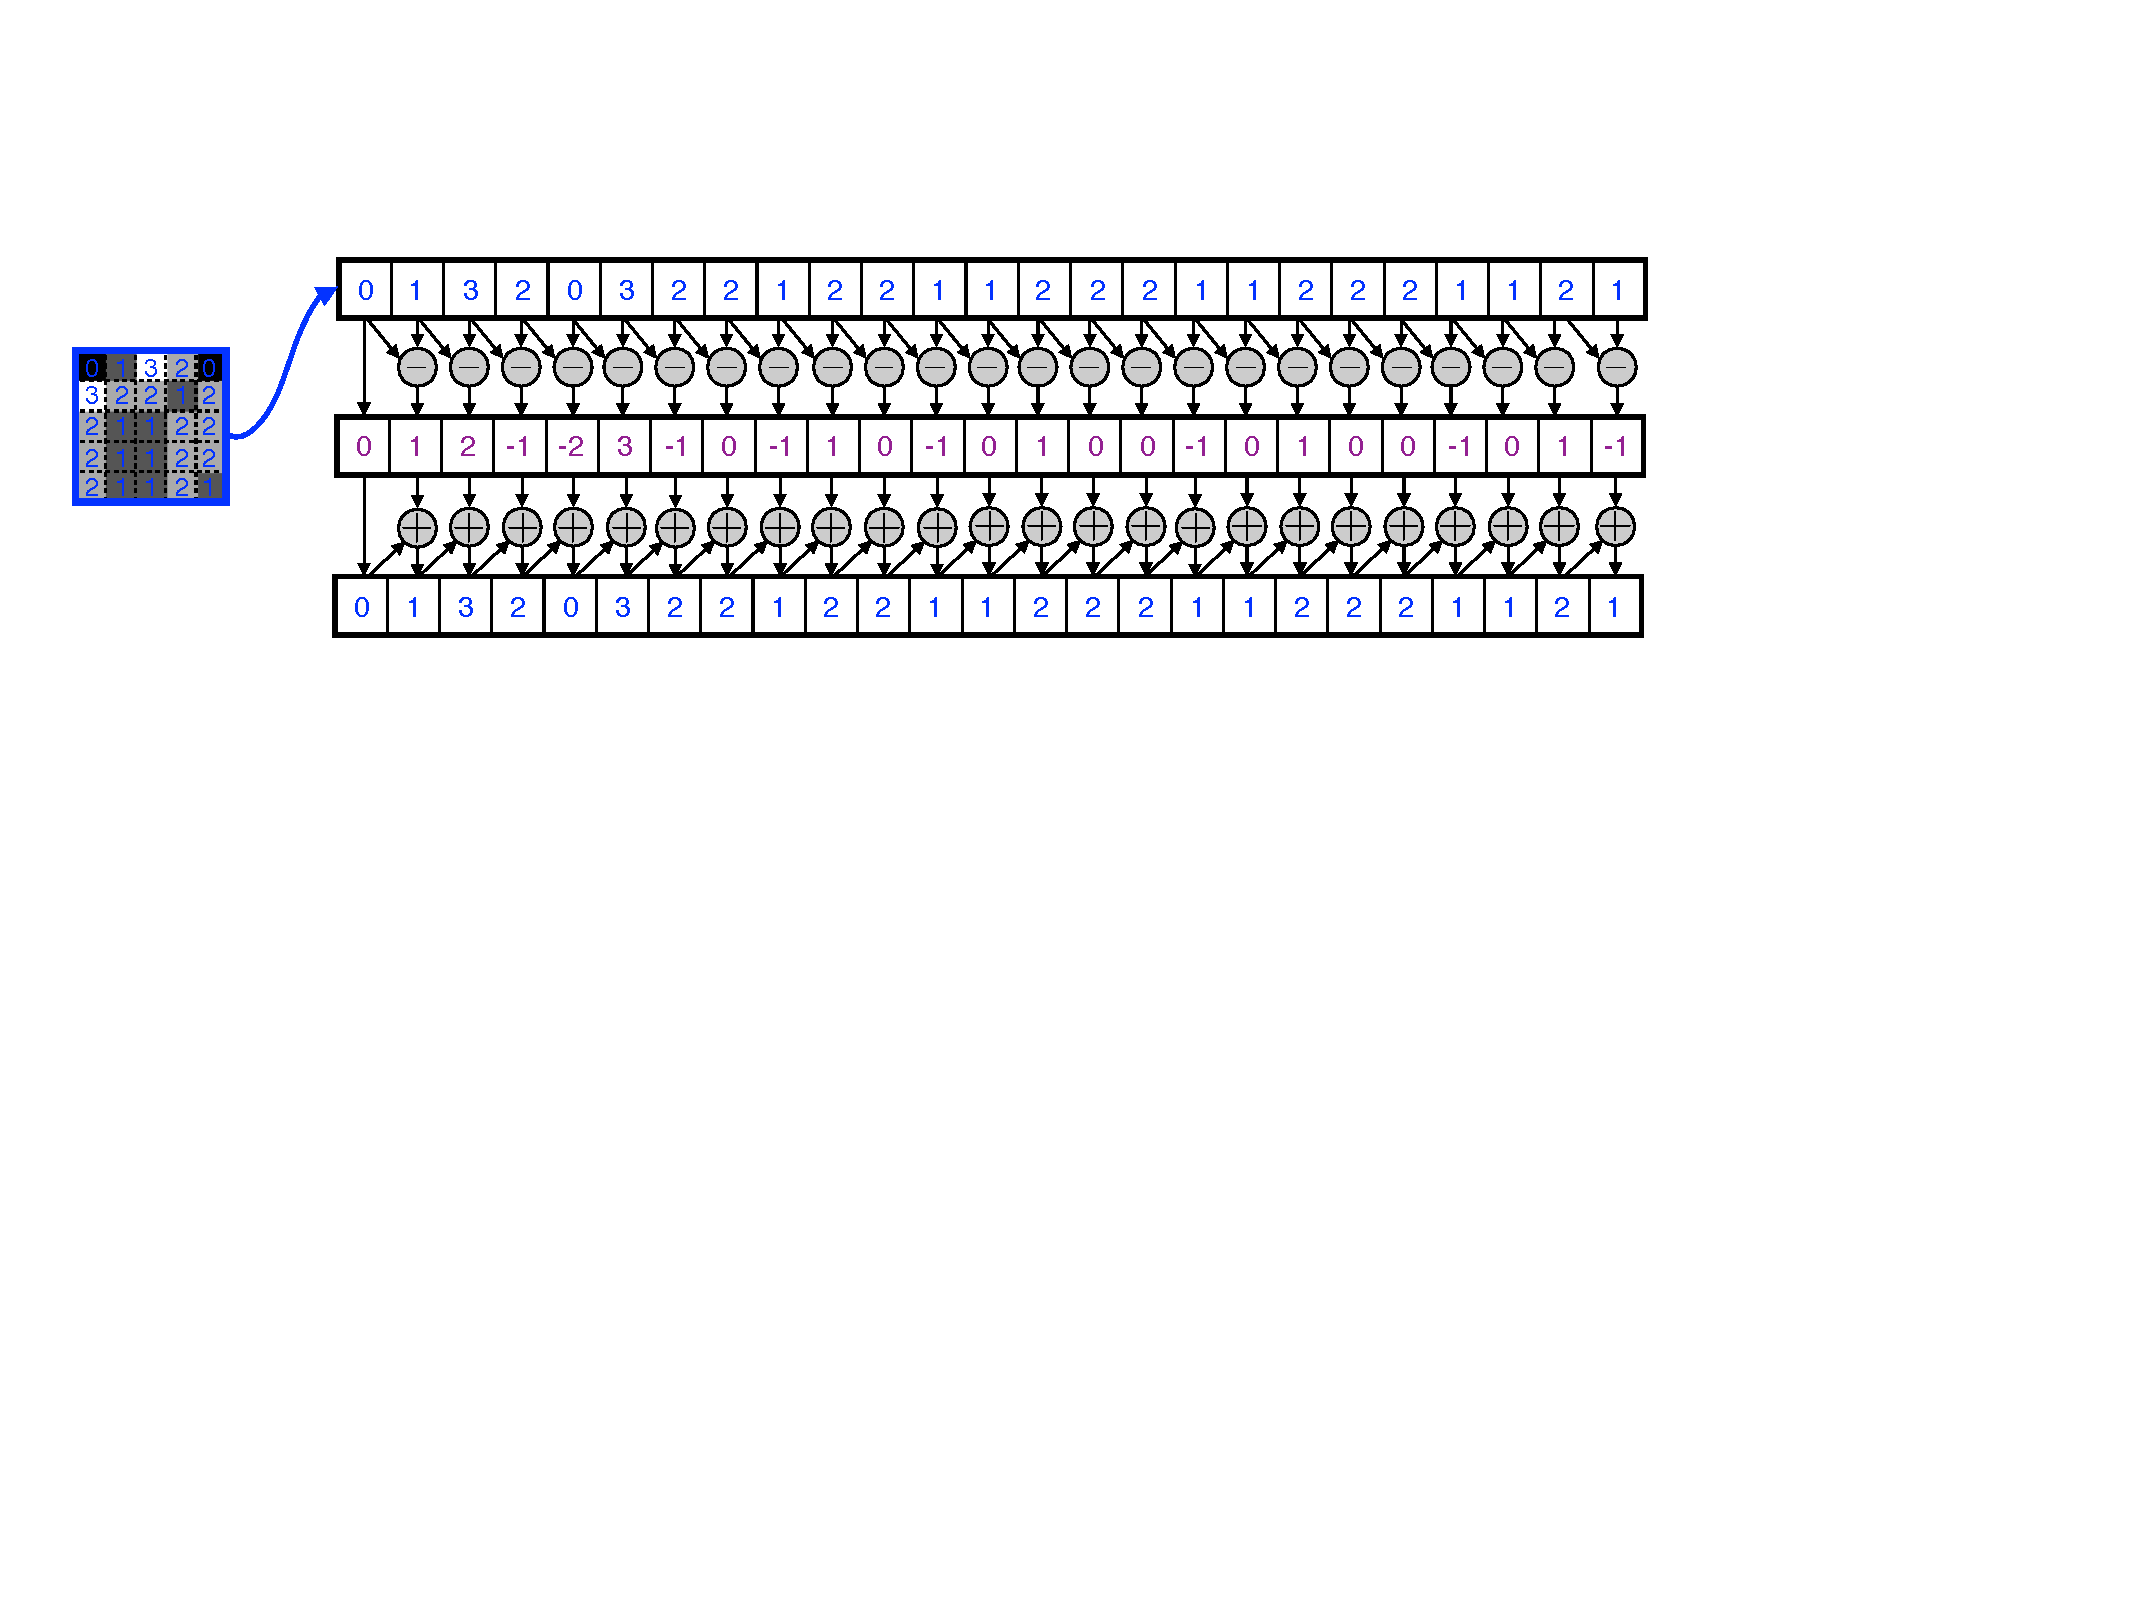
\includegraphics[width=\linewidth]{differences/differences}
}{fig-codage-differences}{Difference representation}


As the pixels can take values $\{\BL{0,1,2,3}\}$, the differences can take the values $\{\GR{-3, \ldots, 3}\}$. In particular, they may be negative (which does not pose any particular problem for defining a coding). The following figure compares the histograms of pixels and differences. We notice that the histogram of the differences is much more \guill{peaked} in the neighborhood of 0, which is logical, because many differences (corresponding to the homogeneous zones) are null or small. The entropy $\mathcal{H}_\Differ$ of the histogram of the differences (which can be modeled with a source $\Differ$) is therefore much lower than the entropy $\mathcal{H} \mot$ of the pixels.

The figure~\ref{fig-entropy-differences} shows a comparison of the histograms of pixel values and differences, calculated over the entire image (and not only on the initial 25 pixel subset).
%
It also shows the tree of an optimal prefix encoding (computed by the Huffman~\cite{Huffman52} algorithm) associated with the histogram of the differences.

\myfig{
\tabTrois{
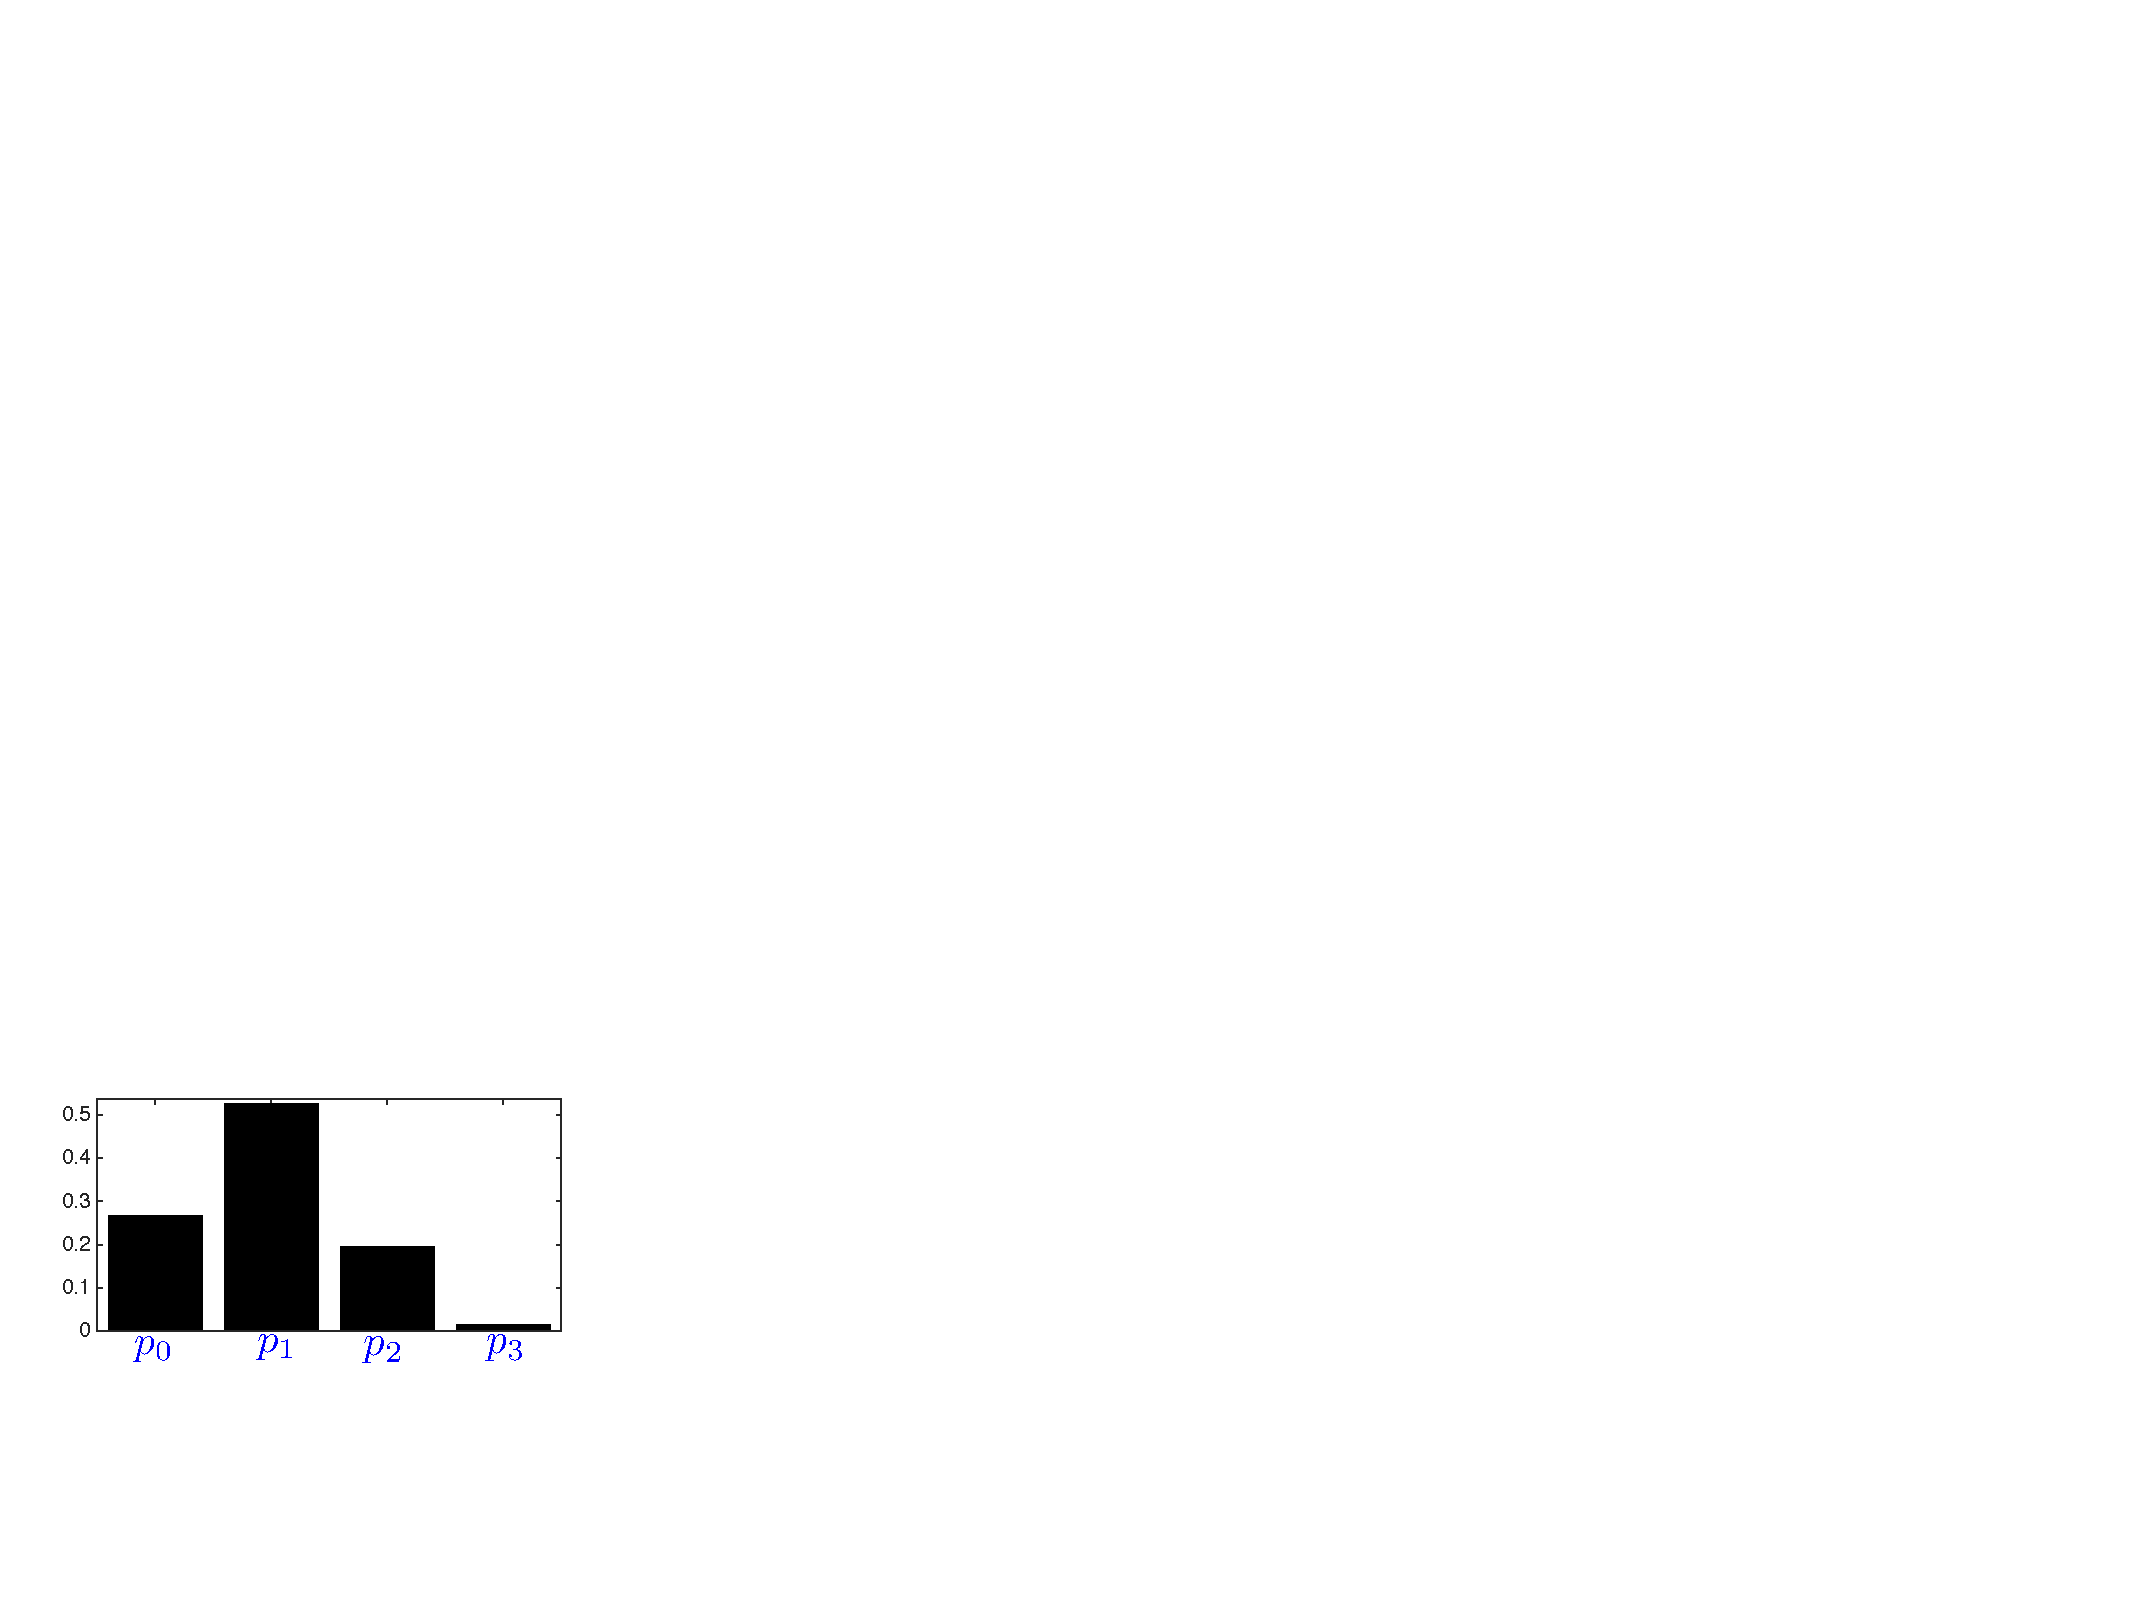
\includegraphics[width=.3\linewidth]{differences/histo-pix}&
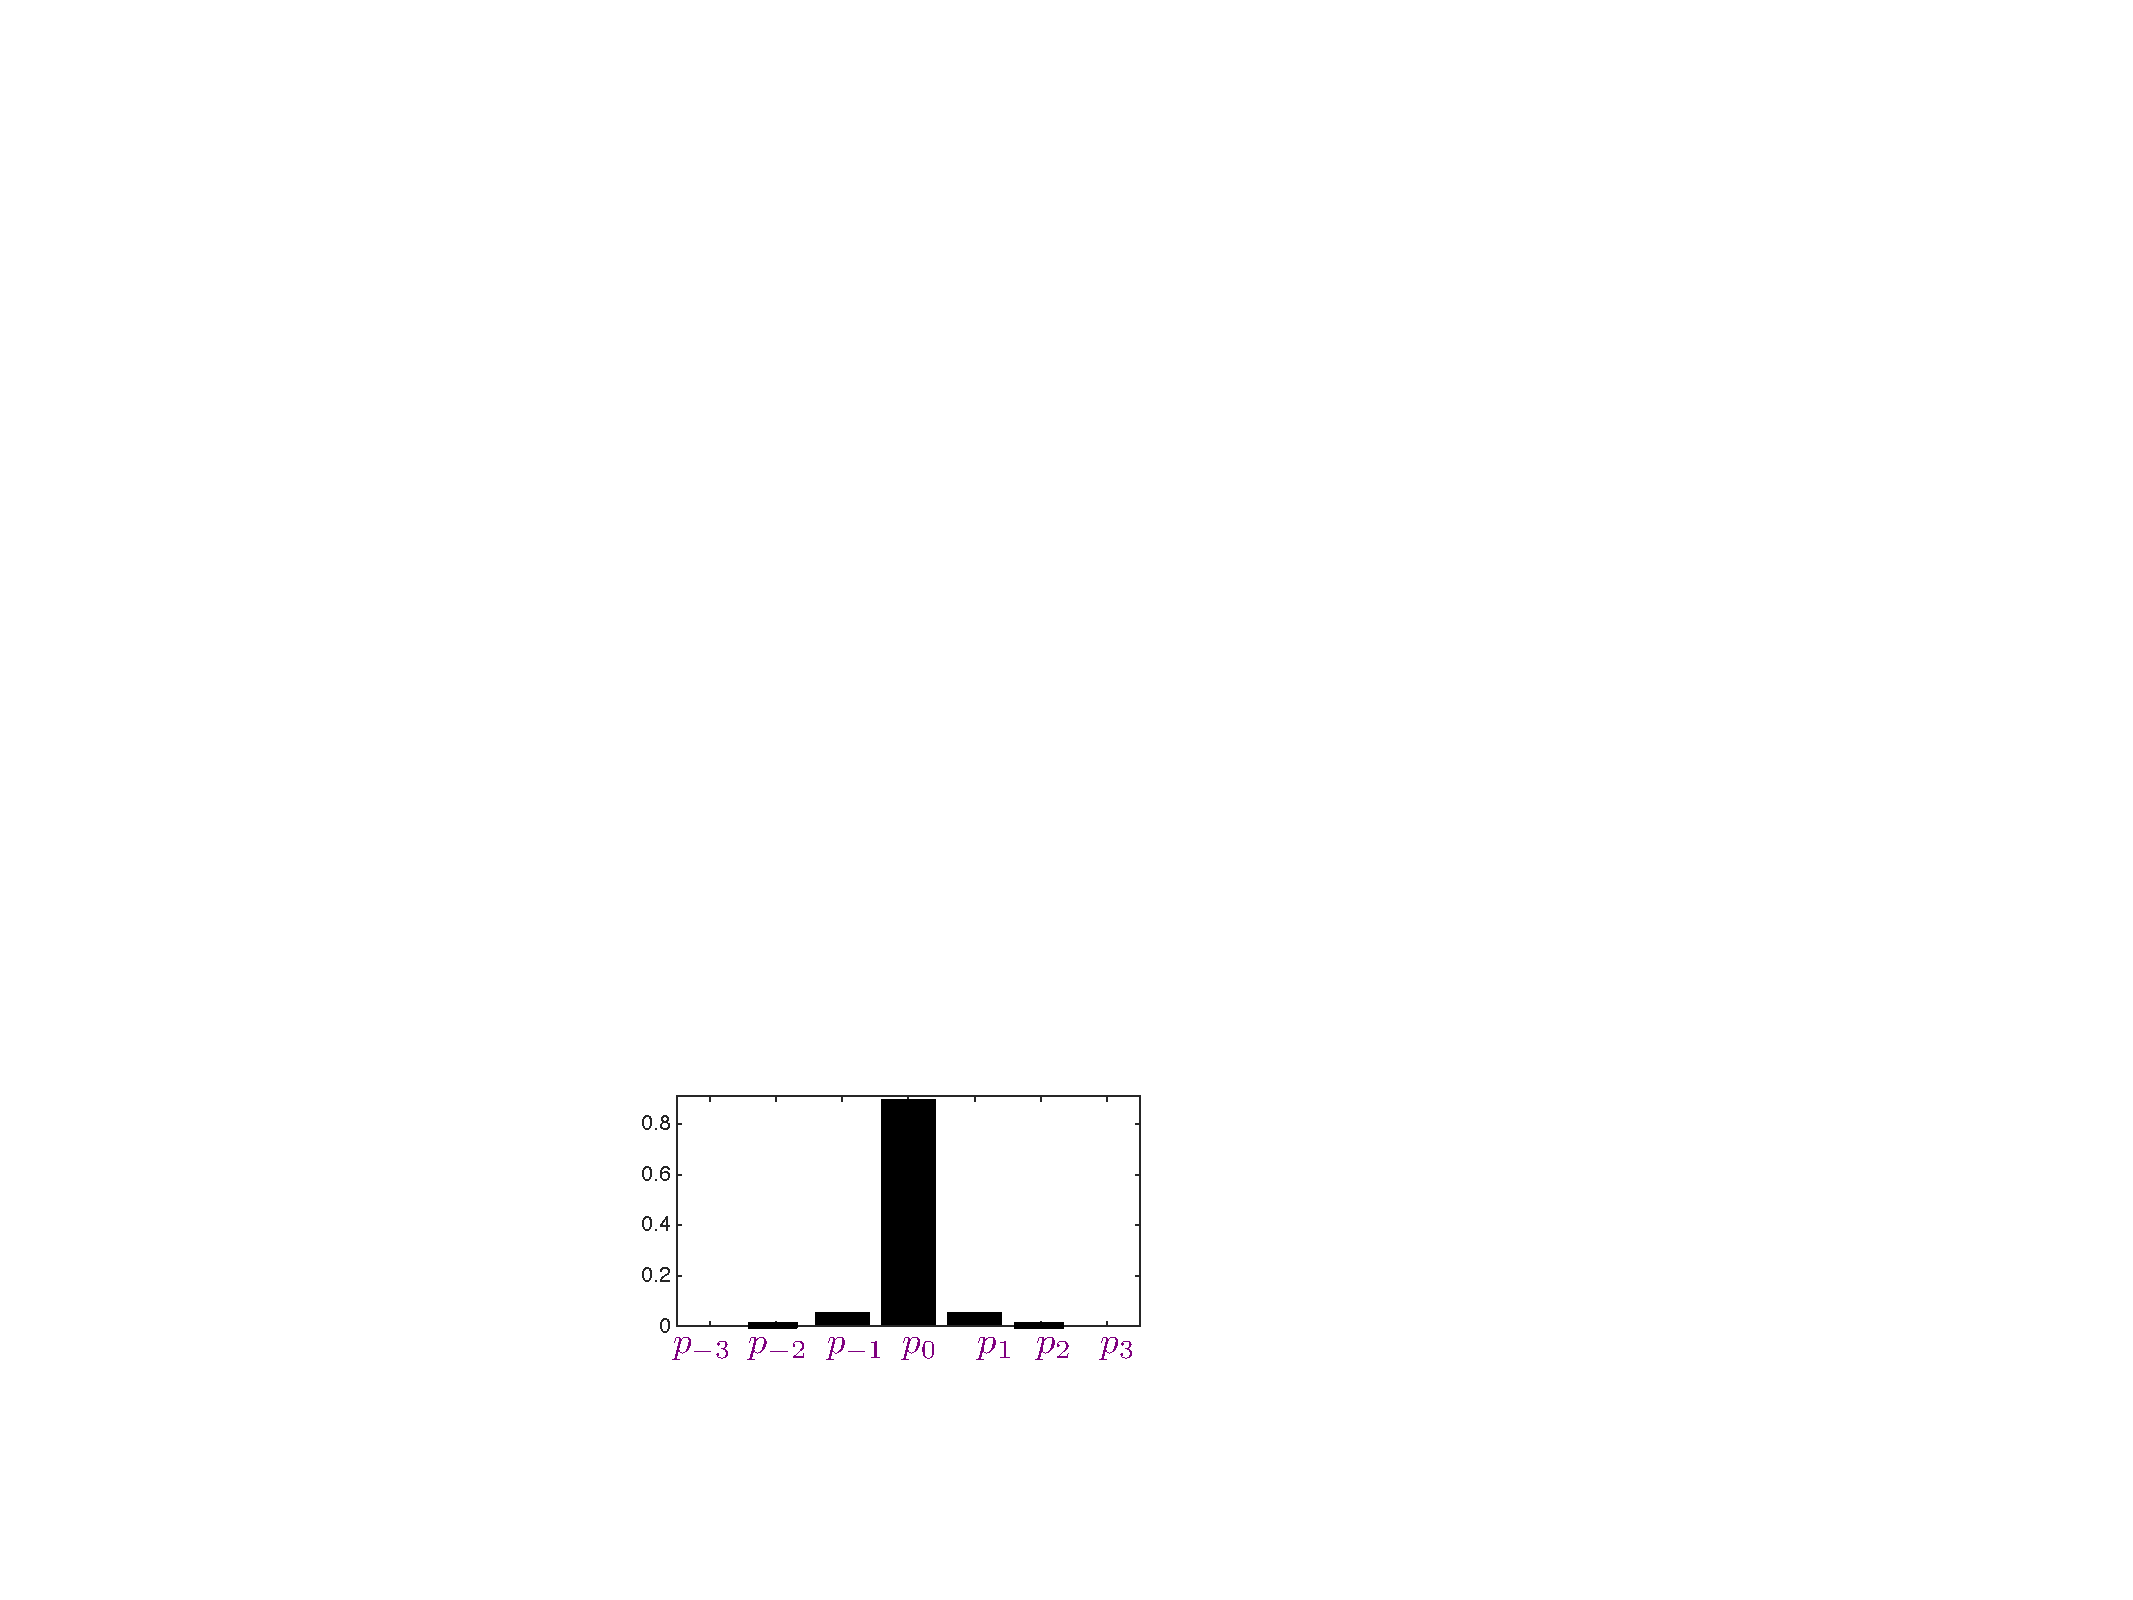
\includegraphics[width=.3\linewidth]{differences/histo-diff}&
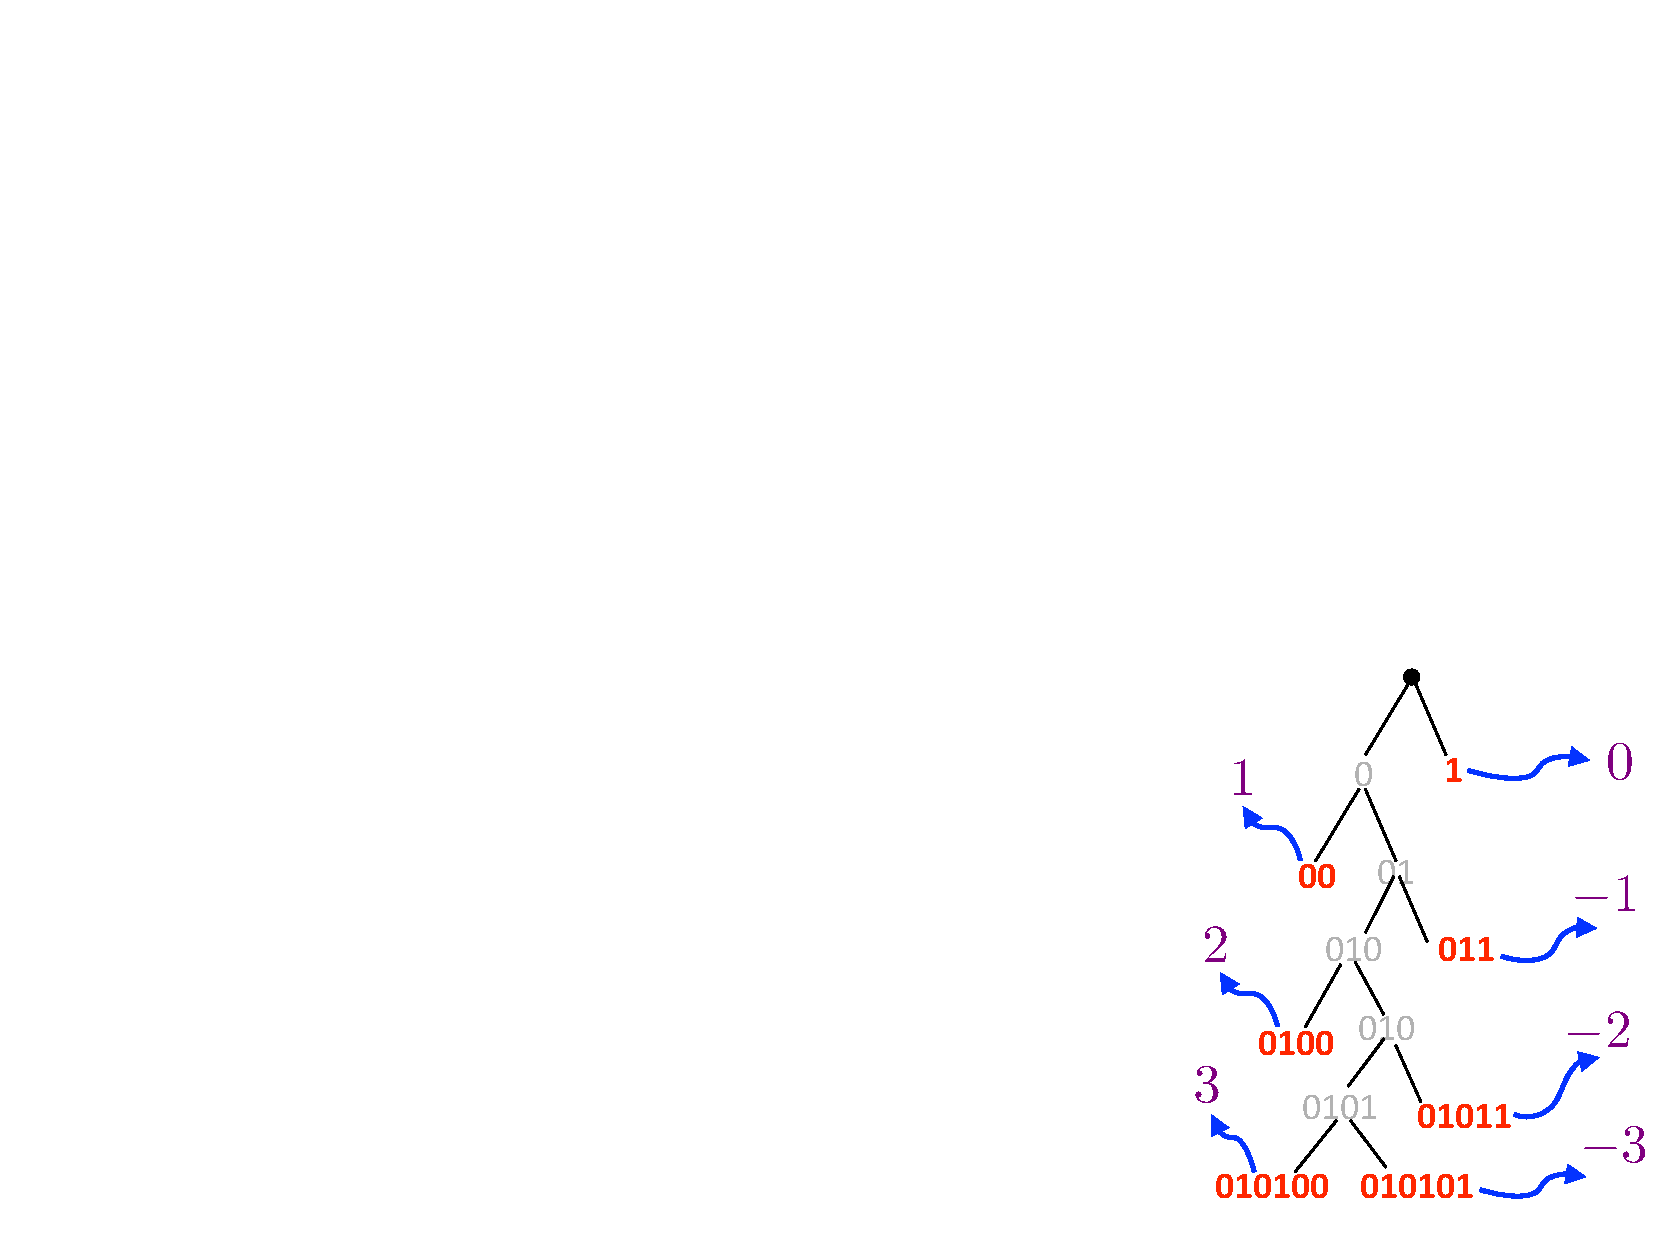
\includegraphics[width=.2\linewidth]{differences/arbre-difference}\\
$\Hh_{\mot} \approx 1.54, \LongMoy \approx 1.67 $ & $\Hh_{\Differ} \approx 0.61, \LongMoy \approx 1.16 $ & Coding Tree
}
}{fig-entropy-differences}{Comparison of histograms of pixel values and differences, and a code tree for these differences. }


This tree corresponds to the coding
$$
	\GR{-3} \mapsto \RE{010101},
	\GR{-2} \mapsto \RE{01011},
	\GR{-1} \mapsto \RE{011},
	\GR{0} \mapsto \RE{1},
	\GR{1} \mapsto \RE{00},
	\GR{2} \mapsto \RE{0100},
	\GR{3} \mapsto \RE{010100}.
$$
This encoding has an average length $\mathcal{L} \approx 1.16$ bits. This average number corresponds well to the entropy boundary and is significantly smaller than the mean length associated with the pixel histogram (1.67 bits), which is itself smaller than the mean length associated with a ($\log_2(4)=2 $ bits). If we pass these lengths to the encoding of the entire image of $ 256 \times 256 $ in gray level, we get the following gains, where 1 ko=8 $\times$ 1024 bits is a \textit{ kilo byte}.
\eq{
\begin{tabular}{c}
Uniform Encoding \\
16.3 kb
\end{tabular}
\quad \longrightarrow \quad
\begin{tabular}{c}
Encoding pixels \\
13.7 kb
\end{tabular}
\quad \longrightarrow \quad
\begin{tabular}{c}
Coding of differences \\
9.5 kb
\end{tabular}
}

The most efficient methods of image compression use more complex transformations, and exploit in a finer way the local regularity of the images. This is the case of the JPEG-2000\mylink{https://fr.wikipedia.org/wiki/JPEG_2000} compression method, which is considered to be the most efficient at the moment, using the wavelets \mylink{https://en.wikipedia.org/wiki/Ondelette}, see the book~\cite{mallat2009a-wav} for more details. There are many other cases where non-independence of symbols can be used to improve coding performance. An important example is the sequence of letters that compose a text.


%%%%%%%%%%%%%%%%%%%%%%%%%%%%%%%%%%%%%%%%%%%%%%%%%% %%%%%%%%%%%%%%%%%%%%%%%%%%%%%%%%
%%%%%%%%%%%%%%%%%%%%%%%%%%%%%%%%%%%%%%%%%%%%%%%%%% %%%%%%%%%%%%%%%%%%%%%%%%%%%%%%%%
%%%%%%%%%%%%%%%%%%%%%%%%%%%%%%%%%%%%%%%%%%%%%%%%%% %%%%%%%%%%%%%%%%%%%%%%%%%%%%%%%%
\section{Conclusion}

The mathematical theory initiated by Claude Shannon defines a framework of thought necessary for the development of effective techniques for the acquisition, processing, storage and transmission of data in digital form. It was these techniques that revolutionized communications and computing during the second half of the 20th century, and enabled the growth of the Internet at the beginning of the 21st century. Without the revolutionary contributions of Shannon, you could not go on vacation with your entire library in your electronic reader, and all episodes of \textit{Game of Thrones} on your tablet!

For more details on the theory of information, we can look at~\cite{CoverThomas}, for its use in signal and image processing, we can look at~\cite{mallat2009a-wav}.
The computer codes used to reproduce the figures in this article are available online at \mylink{https://github.com/gpeyre/2016-shannon-theory}, and other codes are available on the site \url{www.numerical-tours.com}~\cite{2011-peyre-cise}.

%%%%%%%%%%%%%%%%%%%%%%%%%%%%%%%%%%%%%%%%%%%%%%%%%% %%%%%%%%%%%%%%%%%%%%%%%%%%%%%%%%
%%%%%%%%%%%%%%%%%%%%%%%%%%%%%%%%%%%%%%%%%%%%%%%%%% %%%%%%%%%%%%%%%%%%%%%%%%%%%%%%%%
%%%%%%%%%%%%%%%%%%%%%%%%%%%%%%%%%%%%%%%%%%%%%%%%%% %%%%%%%%%%%%%%%%%%%%%%%%%%%%%%%%
\section*{Glossary}

\newcommand{\glossS}[1]{\item \textbf{#1}}

\begin{rs}
\glossS{Pixel}: location on the square grid of an image, sometimes used to refer to the associated value.
\glossS{Symbol}: element $\mot$ of a finite set, for example $\{0, \ldots, N-1\}$.
\glossS{Code}: $ 0$ and $ 1 $ sequence used to encode a $\mot$ symbol.
\glossS{Coding}: set of correspondences between $\mot$ symbols and associated codes, for example $\BL{2} \mapsto \RE{10}$. Also refers to the action of replacing a sequence of symbols with a set of bits.
\glossS{Empirical distribution}: frequency $p_{\mot}$ of appearance of symbols $\mot$ in the sequence of symbols to be coded.
\glossS{Histogram}: graphical representation of the empirical distribution, which can also by extension designate this distribution.
\glossS{Source}: random variable $\Mot$ modeling the symbols, with the distribution $\mathbb{P}(\Mot=\mot)=p_{\mot}$.
\glossS{Entropy}: $\mathcal{H}_\mot$ is a positive number associated with the source $\Mot$ and depends on its probability distribution $(p_{\mot})_\mot$.
\glossS{Number of mean bits of a sequence:} $\mathcal{L}$ is associated with the encoding of a sequence of symbols.
\glossS{Number of source mean bits:} $\mathcal{L}_\mot$ is associated with the encoding of symbols generated by $\Mot$.
\end{rs}



%%%%%%%%%%%%%%%%%%%%%%%%%%%%%%%%%%%%%%%%%%%%%%%%%% %%%%%%%%%%%%%%%%%%%%%%%%%%%%%%%%
%%%%%%%%%%%%%%%%%%%%%%%%%%%%%%%%%%%%%%%%%%%%%%%%%% %%%%%%%%%%%%%%%%%%%%%%%%%%%%%%%%
%%%%%%%%%%%%%%%%%%%%%%%%%%%%%%%%%%%%%%%%%%%%%%%%%% %%%%%%%%%%%%%%%%%%%%%%%%%%%%%%%%
\section *{Acknowledgments}

I thank Marie-No�lle Peyr�, Gwenn Guichaoua, Fran�ois B�guin, G�rard Grancher, Aur�lien Djament and Fran�ois Sauvageot for their careful proofreading of a French version of this text.

The image of the flower is due to Ma�tine Bergounioux. The image of Shannon used for the logo of the article is due to the telehistoriska user of the flickr site (under license CC BY-NC 2.0).



